%--------------------------------------
% Create title frame
\titleframe

%--------------------------------------
% Table of contents
\begin{frame}{Overview}
  \setbeamertemplate{section in toc}[sections numbered]
  \tableofcontents[hideallsubsections]
\end{frame}


\begin{frame}[allowframebreaks]{Classification power system stability (Reminder)}
\begin{quote}
    \textbf{Power system stability is the ability of an electric power system, for a given initial operating condition, to regain a state of operating equilibrium after being subjected to a physical disturbance, with most system variables bounded so that practically the entire system remains intact.} 
    \cite{hatziargyriou2020definition}
\end{quote}
\vspace{0.5cm}
\begin{center}
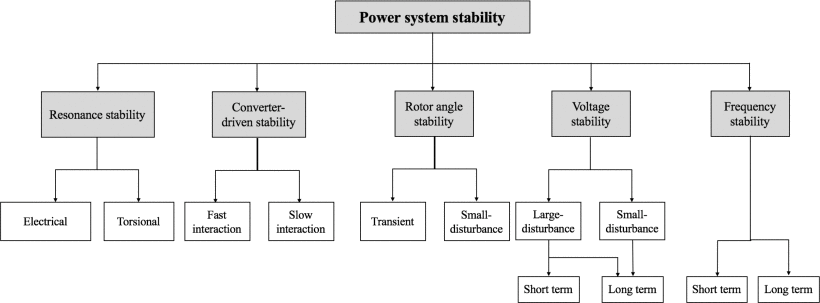
\includegraphics[width=0.9\textwidth]{images/ClassificationStability.png}
\end{center}
\end{frame}

\section{Principle of transient stability}
\begin{frame}[allowframebreaks]{Reminder: generator model and step up transformer}
    \begin{figure}
        \centering
        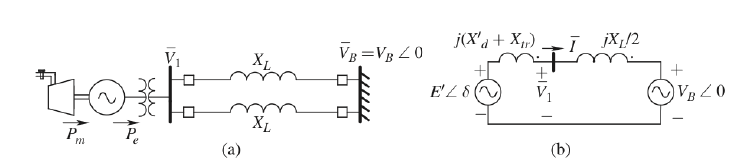
\includegraphics[width=0.9\textwidth]{images/Principle_TS.png}
        \caption{Generator with step-up transformer connected to infinite bus through two parallel lines.}
        \label{fig:OMIB}
    \end{figure}
\begin{itemize}
    \item Consider a generator bus connected through a transformer to a infinite bus system ($\bar{V}_B = V_B$ is an ideal voltage source).
    \item The mechanical power delivered through the shaft is $P_m$.
    \item The electrical power delivered to the grid is denoted $P_e$.
    \item In steady-state, the synchronous machine is modelled as a constant voltage source $E' e^{j\delta}$ behind its transient reactance $X'_d$.
    \item Finally, $X_{tr}$ is the leackage reactance of the transformer.
\end{itemize}
\end{frame}

\begin{frame}[allowframebreaks]{Reminder: active and reactive power flow on a line}
Consider a simple radial system.
\begin{center}
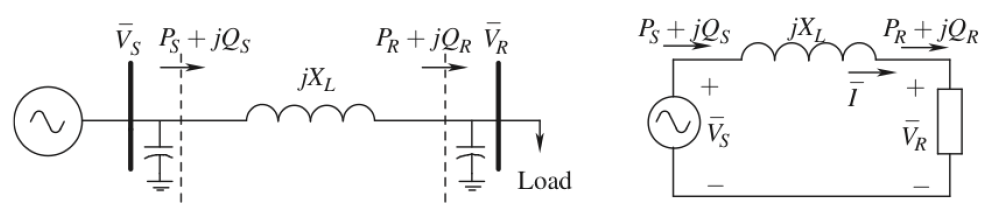
\includegraphics[width=0.7\textwidth]{images/RadialSystem.png}
\end{center}
Assuming no transmission-line losses:
$$S_S = P_S + jQ_S = V_S e^{j \delta_S} \left(\frac{V_S e^{-j \delta_S} - V_R e^{-j \delta_R}}{X}\right) e^{j\frac{\pi}{2}}$$
If we define $\delta = \delta_S-\delta_R$, we have:
$$P_R = P_S = \frac{V_S V_R}{X_L}\sin \delta$$
$$Q_{R} = \frac{V_S V_R \cos \delta}{X_L} - \frac{V^2_R}{X_L}$$
$$Q_{S} = \frac{V_S^2}{X_L} - \frac{V_S V_R \cos \delta}{X_L}$$
\end{frame}

\begin{frame}{Reminder: Electrical power vs. angle}
Plugging the generator and transformer models in the previous models, 
the electrical power $P_e$ is expressed as follows:
\begin{equation}
P_e = \frac{E' V_B}{X_{tr}+X'_d + X_L/2} \sin(\delta)    \label{eq:P_e_delta}
\end{equation}

At equilibrium, $P_e = P_m$. For given reactances and voltage sources, one has:
$$\delta_{eq} = \arcsin\left(P_m \frac{X_{tr}+X'_d + X_L/2}{E' V_B}\right)$$
\end{frame}

\begin{frame}{Reminder: Electrical power vs. angle, graphically}
    \begin{columns}
    \begin{column}{0.55\textwidth}
    \begin{center}
    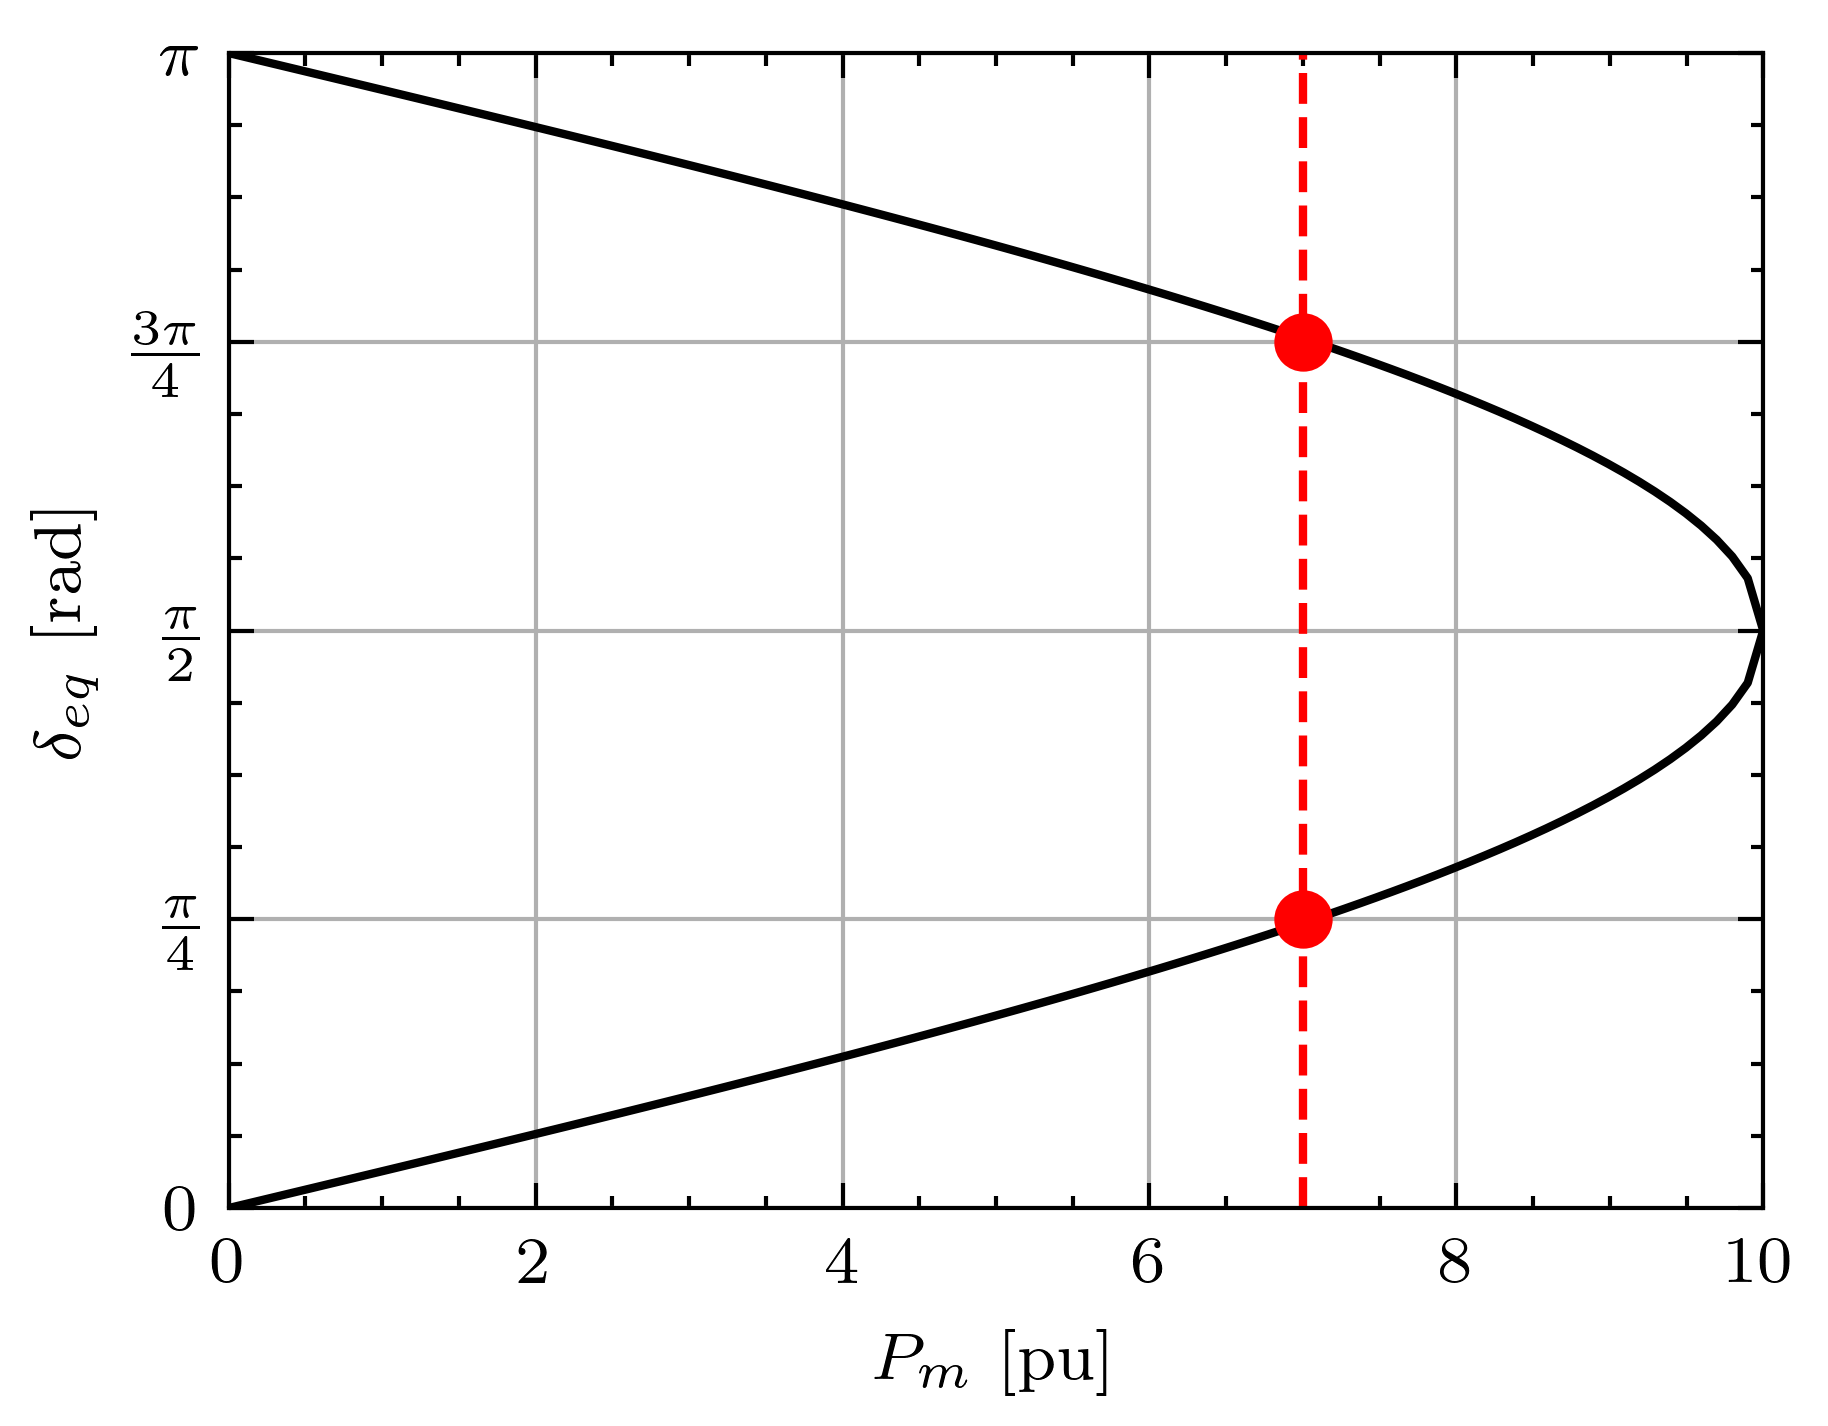
\includegraphics[width=0.9\textwidth]{images/delta_P_m.png}
    \end{center}
    \end{column}
    \begin{column}{0.45\textwidth}

    \begin{itemize}
        \item When we increase $P_{m}$, the electrical angle at equilibrium also increases. 
        \item The maximum value is reached for $\delta_{eq} = \frac{\pi}{2}$.
        \item There exist 
            \begin{itemize}
                \item \textbf{TWO} equilibrium points for $P_m \in [0,10)$
                \item  \textbf{ONE} for $P_m = 10$
                \item  \textbf{NONE} for $P_m>10$.
            \end{itemize}
    \end{itemize}
    \end{column}
\end{columns}


\end{frame}

\begin{frame}[allowframebreaks]{Reminder: what if $P_m$ exceeds $P_e$?}

(In this case,  $P_m > 10.$)

\begin{center}
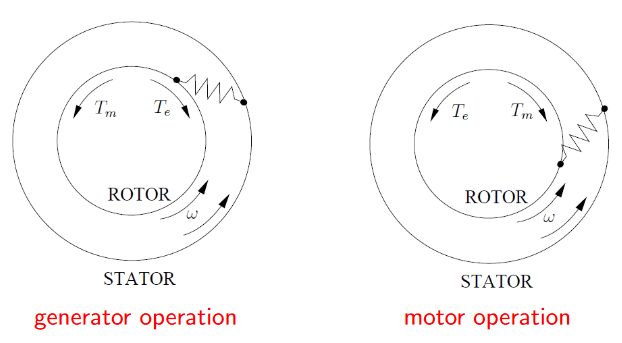
\includegraphics[width=0.6\textwidth]{images/Angle_MechanicAnalogy.png}
\end{center}
\begin{itemize}
    \item In synchronous machines, the rotor rotates at the same angular speed as the magnetic field produced by the stator.
    \item If we denote $\omega_m$ the rotor angular speed and $\omega_s = 2\pi f_s$ the synchronous speed, then $\omega_m = \omega_s$.
    \item The field produced by the rotor and the stator tend to align. 
    \item If they are not aligned, an electromechanical torque is produced. 
    \item This misalignment is represented by the electrical angle: a greater angle induces a larger torque. 
    \item \textbf{BUT} if the angle is too large, the machine loses synchronism and the torque becomes 0.
\end{itemize}
\end{frame}

\begin{frame}{Principle of transient stability}
\begin{columns}
    \begin{column}{0.5\textwidth}
        Consider equation (\ref{eq:P_e_delta}) again:
        $$P_e = \frac{E' V_B}{X_{tr}+X'_d + X_L/2} \sin(\delta)$$

        with (all in per unit)
        \begin{itemize}
            \item $E' = 1.1$, $V_B = 1$, $X_{tr} = 0.8$, $X'_d = 0.4$ 
            \item various values of $X_L = [0.5,1,3]$ (see next slide).
        \end{itemize}
    \end{column}
    \begin{column}{0.5\textwidth}
        \begin{center}
        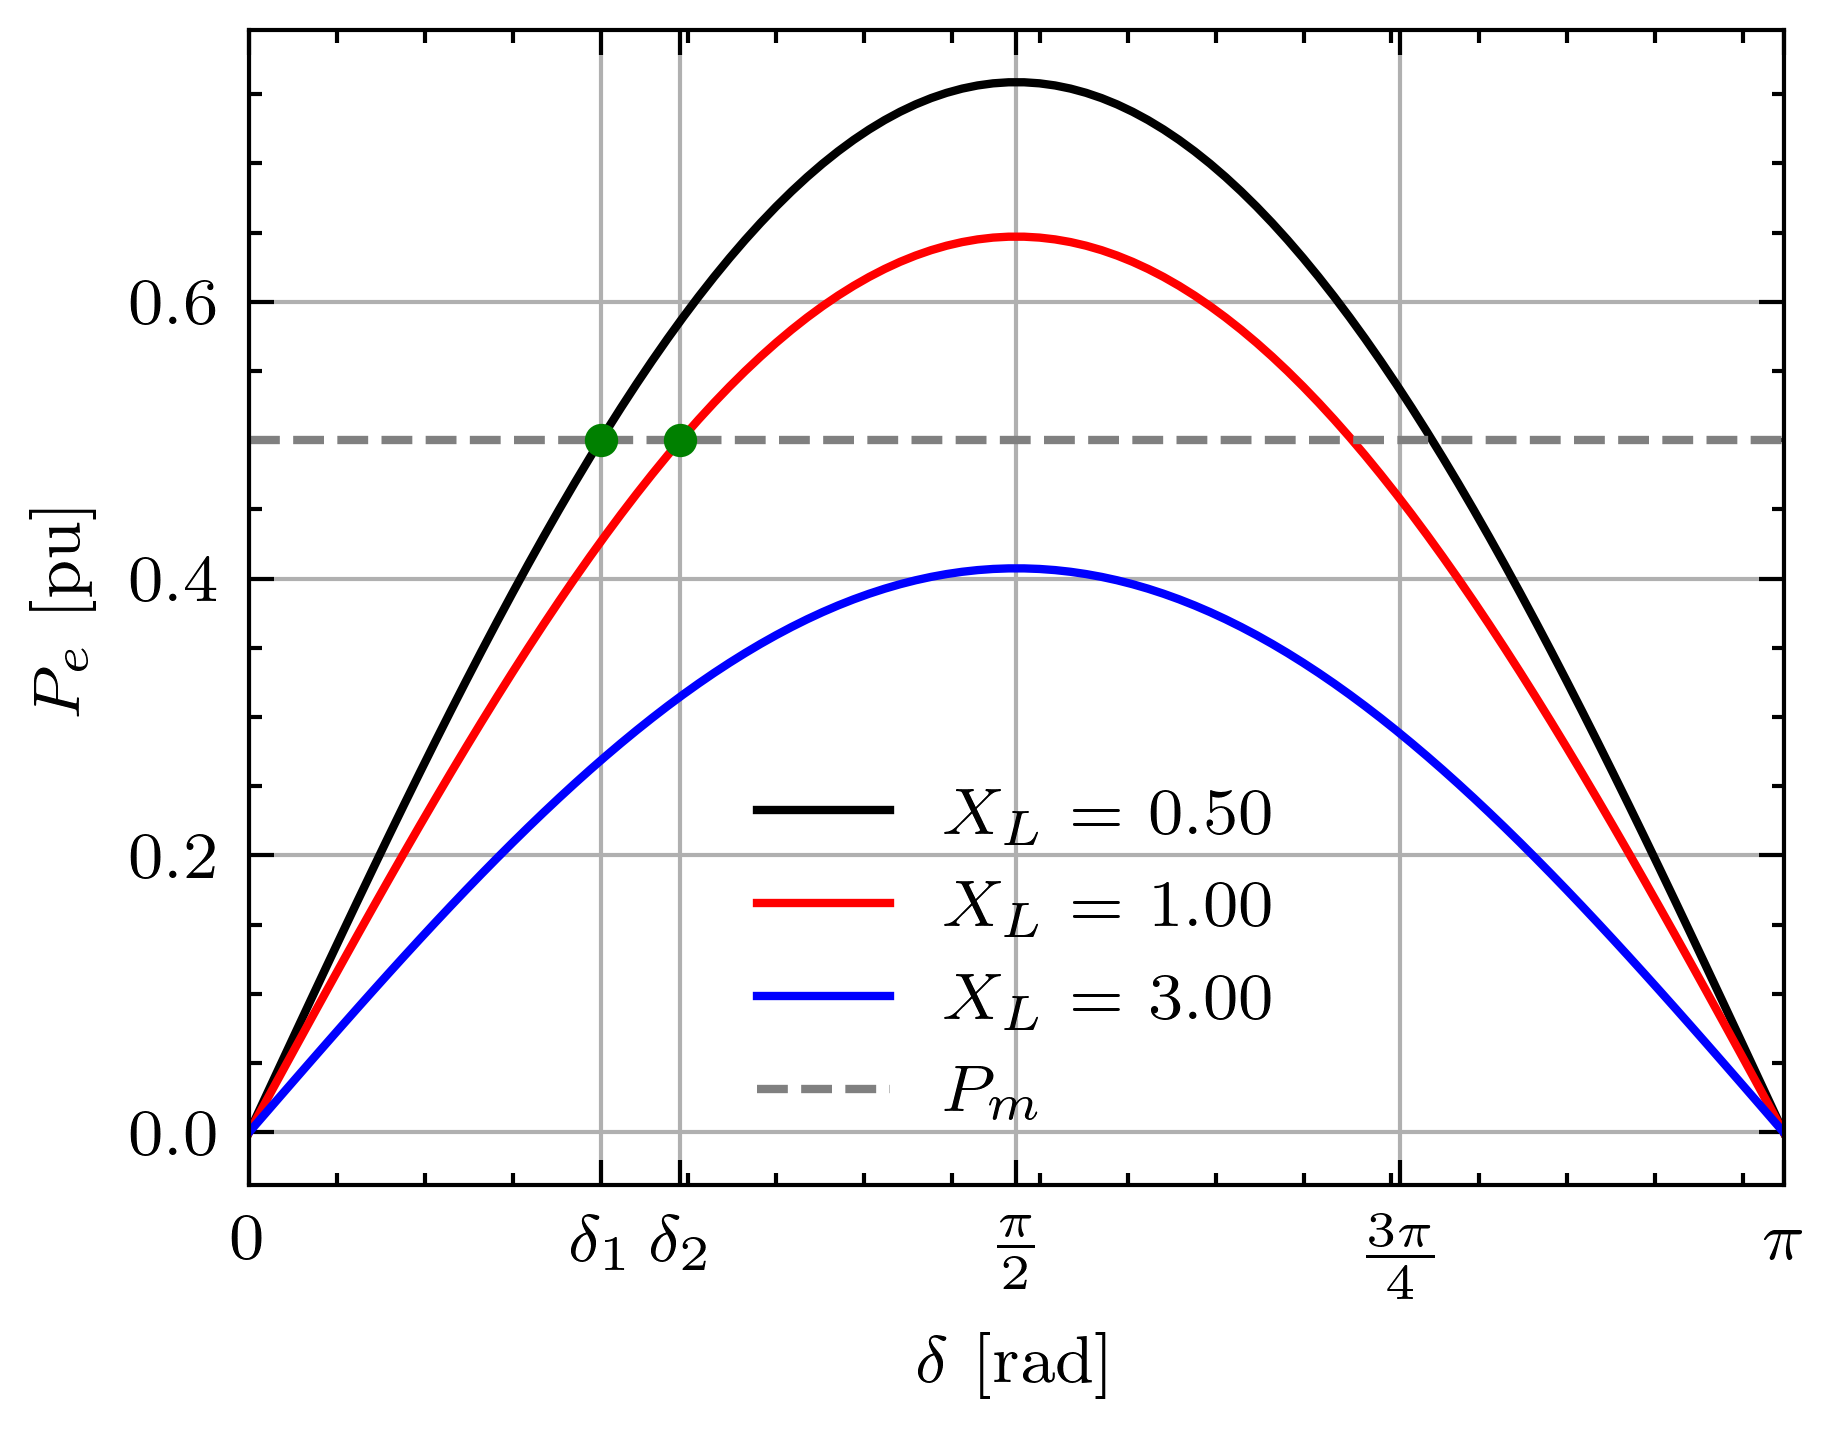
\includegraphics[width=0.95\textwidth]{images/P-delta.png}
        \end{center}
    \end{column}
\end{columns}
\end{frame}

\begin{frame} {Let us consider the following sequence of actions}

\begin{columns}
\begin{column}{0.6\textwidth}
Refer to Figure~\ref{fig:OMIB}:
\begin{enumerate}
    \item \textbf{Pre-fault conditions}: the impedance between the generator and the infinite bus system is $jX_L = j 0.5$ pu.
    \item \textbf{During-fault conditions}: one line is short-circuited, the impedance becomes $jX_L = j 3$ pu.
    \item \textbf{Post-fault conditions}: the short-circuit is cleared by disconnecting a line, the impedance becomes $jX_L = j 1$ pu.
\end{enumerate}
\end{column}
\begin{column}{0.4\textwidth}
For the system to be stable, the system has to stabilize at $\delta = \delta_2$ after the fault occured. \textit{Why?}\\[\baselineskip]

\emph{We will now look at how the system moves from the equilibrium point $\delta_1$ to equilibrium point $\delta_2$}
\end{column}
\end{columns}
\end{frame}

\section{The Swing equation}
\begin{frame} [allowframebreaks]{The swing equation}
Let us define the following quantities; $J_m$ is the moment-of-inertia of the rotational system, $T_m$ is the mechanical torque, $T_e$ is the electrical torque, $\omega_m$ is the rotor speed and $\delta_m$ the rotor angle (in mechanical radians). Using Newton's Second Law, one has:
$$J_m\frac{d^2\delta_m}{dt^2} = T_m-T_e$$
Multiplying both sides by $\omega_m$ (the rotor speed), one has:
$$\omega_m J_m \frac{d^2\delta_m}{dt^2} = P_m-P_e$$
We then define
$$H_{gen} = \frac{\frac{1}{2}J_m \omega_{syn,m}^2}{S_{rated,gen}} = \left[\frac{kg \cdot m^2 \times 1/s^2}{kg \cdot m^2/s^3}\right] = \left[s\right]$$
where $\omega_{syn,m}$ is the synchronous speed (in mechanical radians/s), $S_{rated,gen}$ the nominal rated size of the generator.

\begin{block}{About the inertia constant $H_{gen}$}
The inertia constant of a machine $H_{gen}$ is a value that quantifies how much kinetic energy is stored in the rotating mass of a machine relative to its power rating. 
It indicates the duration for which a machine can supply its rated power using only its stored rotational kinetic energy when the input power is suddenly removed.
It takes a value in a range of 
\begin{itemize}
    \item 3 to 11s for turbo-alternators
    \item 1 to 2s  for hydro generators.
\end{itemize} 
\end{block}


One can write the swing equation by substituing $J_m$ by $H_{gen}$:
$$\left(\frac{\omega_m}{\omega_{syn,m}^2}\right)2 H_{gen} \frac{d^2\delta_m}{dt^2} = P_{m,gen,pu} - P_{e,gen,pu}$$
where $P_m$ and $P_e$ are in per-unit of the generator MVA base. One can also write the equation in the system base $S_{system}$:
$$\left(\frac{\omega_m}{\omega_{syn,m}^2}\right)2 H \frac{d^2\delta_m}{dt^2} = P_{m,pu} - P_{e,pu}$$
with
$$H = H_{gen} \left(\frac{S_{rated,gen}}{S_{system}}\right)$$
Finally, we make the reasonable assumption that $\omega_m \approx \omega_{syn,m}$, and we express everything in terms of electrical radians.
\begin{equation}
\left(\frac{2H}{\omega_{syn}}\right) \frac{d^2\delta}{dt^2} = P_{m,pu} - P_{e,pu} \label{eq:swing}
\end{equation}

\end{frame}

\begin{frame}{What can we say about the swing equation?}
\begin{itemize}
    \item If the mechanical power provided at the shaft $P_m$ is greater than the electrical power transferred to the network $P_e$, the machine accelerates $\frac{d^2\delta}{dt^2} = \frac{d\Delta\omega}{dt} > 0$, where $\Delta\omega$ is the deviation from the synchronous speed $\omega_{syn}$.
    \item It decelerates if the electrical power is greater than the mechanical power.
    \item The acceleration is proportional to the machine inertia $H$
\end{itemize}
\begin{block}{Question}
    {What is the inertia of PV panels?}
\end{block}
\end{frame}



\begin{frame}[allowframebreaks]{Transient stability using Equal-Area Criterion}
From the swing equation (\ref{eq:swing})
$$\left(\frac{2H}{\omega_{syn}}\right) \frac{d^2\delta}{dt^2} = P_{m,pu} - P_{e,pu}$$
Rearrange the terms and multiply both sides by $d\delta/dt$:
$$2\frac{d\delta}{dt}\frac{d^2\delta}{dt^2} = \frac{\omega_{syn}}{H}\left(P_{m,pu}-P_{e,pu}\right)\frac{d\delta}{dt}$$
Applying change of variables $\delta = \theta$, and integrating both sides between $\delta_0$ and an arbitrary angle $\delta$:
$$\int_{\delta_0}^{\delta} \left(2\frac{d\theta}{dt}\frac{d^2\theta}{dt^2}\right) dt = \frac{\omega_{syn}}{H}\int_{\delta_0}^{\delta} \left(P_{m,pu}-P_{e,pu}\right)d\theta$$
Assume $\delta_0$ being an equilibrium point, \emph{i.e.} $d\delta/dt|_{\delta = \delta_0} = 0$, we have:
$$\left(\frac{d\delta}{dt}\right)^2 = \frac{\omega_{syn}}{H}\int_{\delta_0}^{\delta} \left(P_{m,pu}-P_{e,pu}\right) d\theta$$


The left term $\left(\frac{d\delta}{dt}\right)^2 = \Delta\omega^2$ represents the kinetic energy of the machine at an arbitrary angle $\delta^*$ (with respect to the synchronous speed $\omega_{syn}$) $\rightarrow$ rotational kinetic energy: $\frac{1}{2} J \omega^2$ with $J$ the moment-of-inertia and $\omega$ the angular speed.
As long as $P_{m,pu} > P_{e,pu}$, the machine gains kinetic energy and accelerates. For the system to stabilize, it must exist an angle $\delta_{m}$ at which the kinetic energy becomes 0, and thus:
$$\int_{\delta_0}^{\delta} \left(P_{m,pu}-P_{e,pu}\right) d\theta = 0$$
Let us consider the following system; at time $t$ and angle $\delta_0$, a short-circuit occurs and is cleared at time $t+t_{cl}$ and angle $\delta_{cl}$ by tripping the line.
\begin{center}
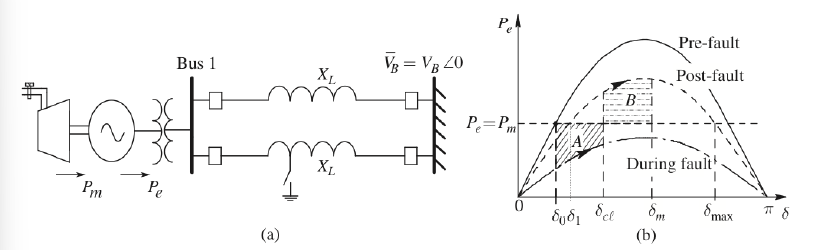
\includegraphics[width=0.9\textwidth]{images/TransientStabilityEAC.png}
\end{center}

For a stable system, we highlighted that:
$$\int_{\delta_0}^{\delta} \left(P_{m,pu}-P_{e,pu}\right) d\theta = 0$$
For our little example, one can write the same condition:
$$\underbrace{\int_{\delta_0}^{\delta_{cl}} \left(P_{m,pu}-P_{e,fault,pu}\right) d\theta}_{\text{Area A}} - \underbrace{\int_{\delta_{cl}}^{\delta_{m}} \left(P_{e,post-fault,pu}-P_{m,pu}\right) d\theta}_{\text{Area B}} = 0$$
During the first part (Area A), the machine accelerates. After the fault (Area B), the machine decelerates and the net acceleration becomes 0. At angle $\delta_{m}$, there is still a mismatch between the electrical power and the mechanical power, thus the machine swings back (from $\delta_{m}$ to $\delta_{2}$).
\begin{center}
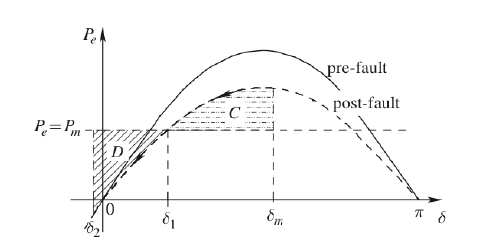
\includegraphics[width=0.6\textwidth]{images/SwingsBack.png}
\end{center}

Without any damping (kinetic energy losses), the system oscillates indefinitely between angle $\delta_2$ and $\delta_m$.
\begin{center}
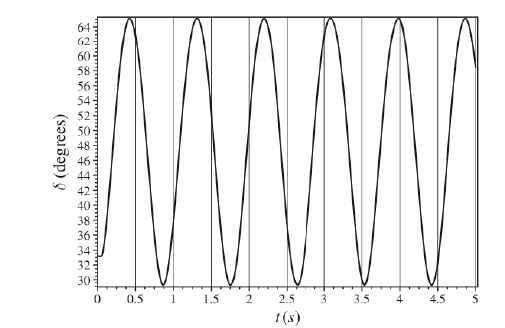
\includegraphics[width=0.6\textwidth]{images/RotorOscillation.png}
\end{center}
However, in a real system, the damping would cause the machine to settle down at an angle $\delta_1$ (new equilibrium point).
Synchronous machines have \emph{damper windings}. In perfect steady state, the magnetic fields produced by both the stator and the rotor are fixed relative to the rotor so there is no current in the dampers. On the other hand, if the rotor moves with respect to the magnetic field, the current induced in the dampers create a damping torque according to Lenz's law.
\end{frame}

\begin{frame} {Critical Clearing Angle}
Let us come back to our definition of stability for our little system:
$$\underbrace{\int_{\delta_0}^{\delta_{cct}} \left(P_{m,pu}-P_{e,fault,pu}\right) d\theta}_{\text{Area A}} - \underbrace{\int_{\delta_{cct}}^{\delta_{max}} \left(P_{e,post-fault,pu}-P_{m,pu}\right) d\theta}_{\text{Area B}} = 0$$
\textbf{What are the conditions to ensure there exists $\delta_{cl}$ such that Area A = Area B?}
We introduce the concept of critical clearing angle $\delta_{cct}$. Past this point, Area A will always be greater than Area B, such that the system cannot stabilize. We associate the critical clearing time $CCT$ to the critical clearing angle, \emph{i.e.} the maximum time allowed to clear the fault before the system gets unstable.
\end{frame}

\begin{frame} {Critical Clearing Angle: Visual representation}
\begin{center}
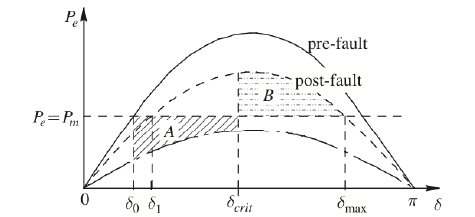
\includegraphics[width=0.6\textwidth]{images/CCT_example.png}
\end{center}
\textbf{Mathematical formulation}
$$\underbrace{\int_{\delta_0}^{\delta_{cct}} \left(P_{m,pu}-P_{e,fault,pu}\right) d\theta}_{\text{Area A}} - \underbrace{\int_{\delta_{cct}}^{\delta_{max}} \left(P_{e,post-fault,pu}-P_{m,pu}\right) d\theta}_{\text{Area B}} = 0$$
One has to determine the angle $\delta_{max}$ such that $P_{e,post-fault} = P_{m}$, and the angle $\delta_{0}$ such that $P_{e,pre-fault} = P_{m}$. Then solving this equation gives $\delta_{cct}$. Finally, using the \textbf{swing equation}, one can determine the critical clearing time $CCT$, \emph{i.e.} the time needed to reach the angle $\delta_{cct}$.
\end{frame}

\section{Practical Example}
\begin{frame}[allowframebreaks]{Problem statement}
Let us consider the following system:
\begin{center}
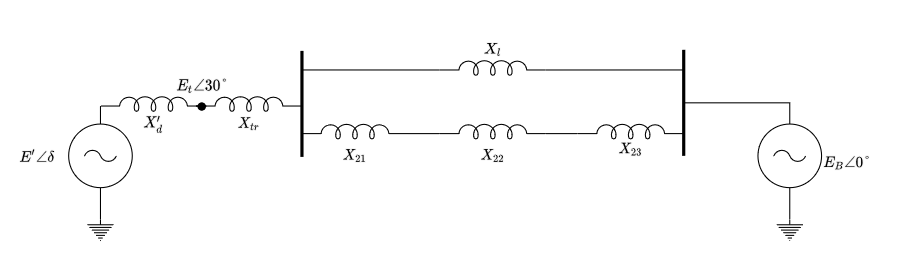
\includegraphics[width=0.9\textwidth]{images/InitialSystem.png}
\end{center}
and the following data:
$$X_d' = 0.3, X_{tr} = 0.5, X_{l} = 1, X_{21} = 0.5, X_{22} = \frac{1}{6}, X_{23} = \frac{1}{3}$$
and
$$\bar{E}_{t} = 1e^{j \pi/6}, \bar{E}_{B} = 1e^{j0}$$
\end{frame}

\begin{frame}[allowframebreaks]{Equivalent}
We can derive the following equivalent:
\begin{center}
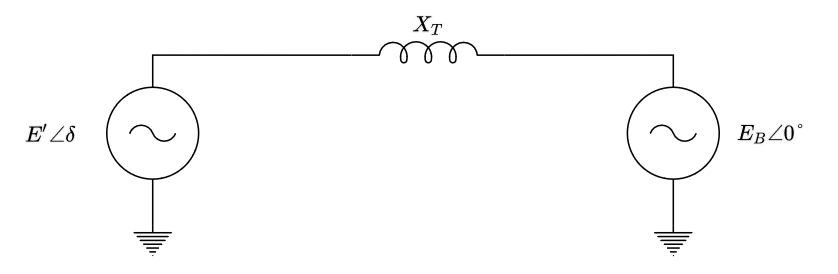
\includegraphics[width=0.9\textwidth]{images/InitialSystemEq.png}
\end{center}
where
$$X_T = X_{tr} + X_{d}' + \frac{X_{l}\left(X_{21}+X_{22}+X_{23}\right)}{X_{21}+X_{22}+X_{23}+X_{l}} = 1.3$$
The power transfer from the machine to the infinite-bus system takes the following form:
$$P = \frac{E' E_{B}}{X_{T}} \sin \delta$$
\end{frame}

\begin{frame}[allowframebreaks]{Find $\bar{E}'$, $P_e$ and $P_m$}
\begin{enumerate}
    \item Current from $\bar{E}_{t}$ to $\bar{E}_{B}$
    $$\bar{I}_{t\rightarrow B} = \frac{\bar{E}_{t}-\bar{E}_{B}}{jX_{T} - jX_{d}'}$$
    \item $\bar{I}_{t\rightarrow B}$ is the same as the one from $\bar{E'}$ to $\bar{E}_{t}$
    $$\bar{E}' = j X_{d}' \bar{I}_{t\rightarrow B} + \bar{E}_{t} = 1.05095 e^{j 38.2057/180}$$
    \item Find $P_e$
    $$P_e = \frac{1.05095\ 1\ \sin(38.2057/180)}{1.3} = 0.5$$
    \item Initially, the system is at equilibrium.
    $$P_m = P_e = 0.5$$
\end{enumerate}
In the following, we will compute the maximum power outputs for three different conditions: Pre-fault, During-Fault and Post-Fault. It will allow us to determine the 3 different $P-\delta$ curves.
\end{frame}

\begin{frame}{Pre-fault condition}
\textbf{We compute the maximum power output while assuming $E'$ does not change.}
\emph{If the transient stability study lasts a second or less, it is reasonable to consider, as a first-order approximation, that the exciter of the synchronous machine cannot respond in such short amount of time. Hence, $E'$ does not change}
\vspace{0.5cm}
\hrule
\vspace{0.5cm}
Maximum power output:
$$\hat{P}_{e,bf} = \frac{E'E_{B}}{X_{T}} = 0.808$$
\end{frame}

\begin{frame}[allowframebreaks]{During-fault condition}
A short-circuit occurs between lines $22$ and $23$. The circuit topology changes and is depicted below.
\begin{center}
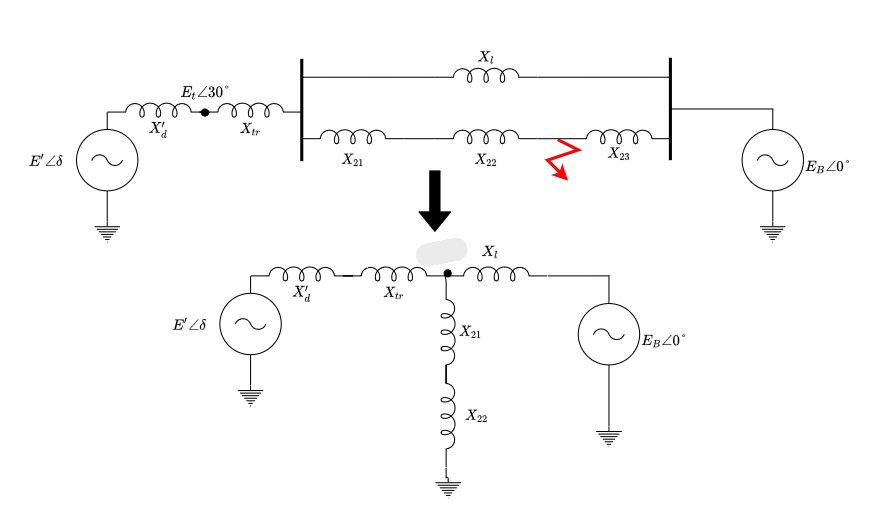
\includegraphics[width=0.7\textwidth]{images/DuringFault.png}
\end{center}
\end{frame}

\begin{frame}[allowframebreaks]{During-fault condition: Thévenin equivalent}
We can derive the following Thevenin's equivalent
\begin{center}
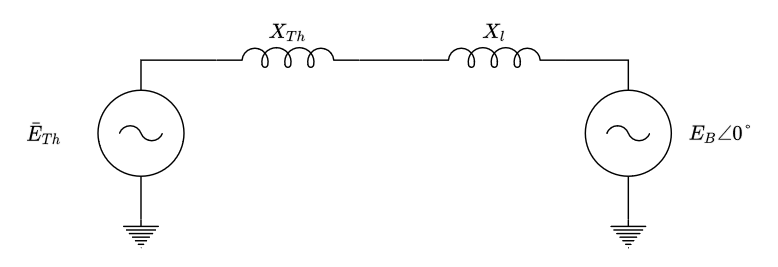
\includegraphics[width=0.6\textwidth]{images/TheveninEquiv.png}
\end{center}
where
$$\bar{E}_{th} = \bar{E'} \frac{X_{21} + X_{22}}{X_{d}+X_{tr} + X_{21} + X_{22}} = 0.478 e^{j 38.206/180}$$
and
$$X_{th} = \frac{1}{\frac{1}{X_d' + X_{tr}}+\frac{1}{X_{21}+X_{22}}} = 0.364$$
and then get the maximum power output:
$$\hat{P}_{e,df} = \frac{E_{th}E_{B}}{X_{th} + X_{l}} = 0.35$$
\end{frame}

\begin{frame}{Post-fault condition}
The line $2$ is tripped to clear the short-circuit.
The impedance of the path connecting the machine to the infinite-bus system becomes $X_d' + X_{tr} + X_{l} = 1.8$.
The maximum power output is:
$$\hat{P}_{e,pf} = \frac{E'E_{B}}{X_d' + X_{tr} + X_{l}} = 0.584$$
\end{frame}

\begin{frame}{Practical Example}
\begin{columns}
    \begin{column}{0.45\textwidth}
        The final $P-\delta$ curves are shown here under, with
        $$\delta_1 = \arcsin \left(\frac{P_m}{\hat{P}_{e,bf}}\right) = 0.667$$ $$\delta_2 = \arcsin \left(\frac{P_m}{\hat{P}_{e,pf}}\right) = 1.028$$ $$ \delta_{max} = 2.114$$
    \end{column}
    \begin{column}{0.55\textwidth}
        \begin{center}
        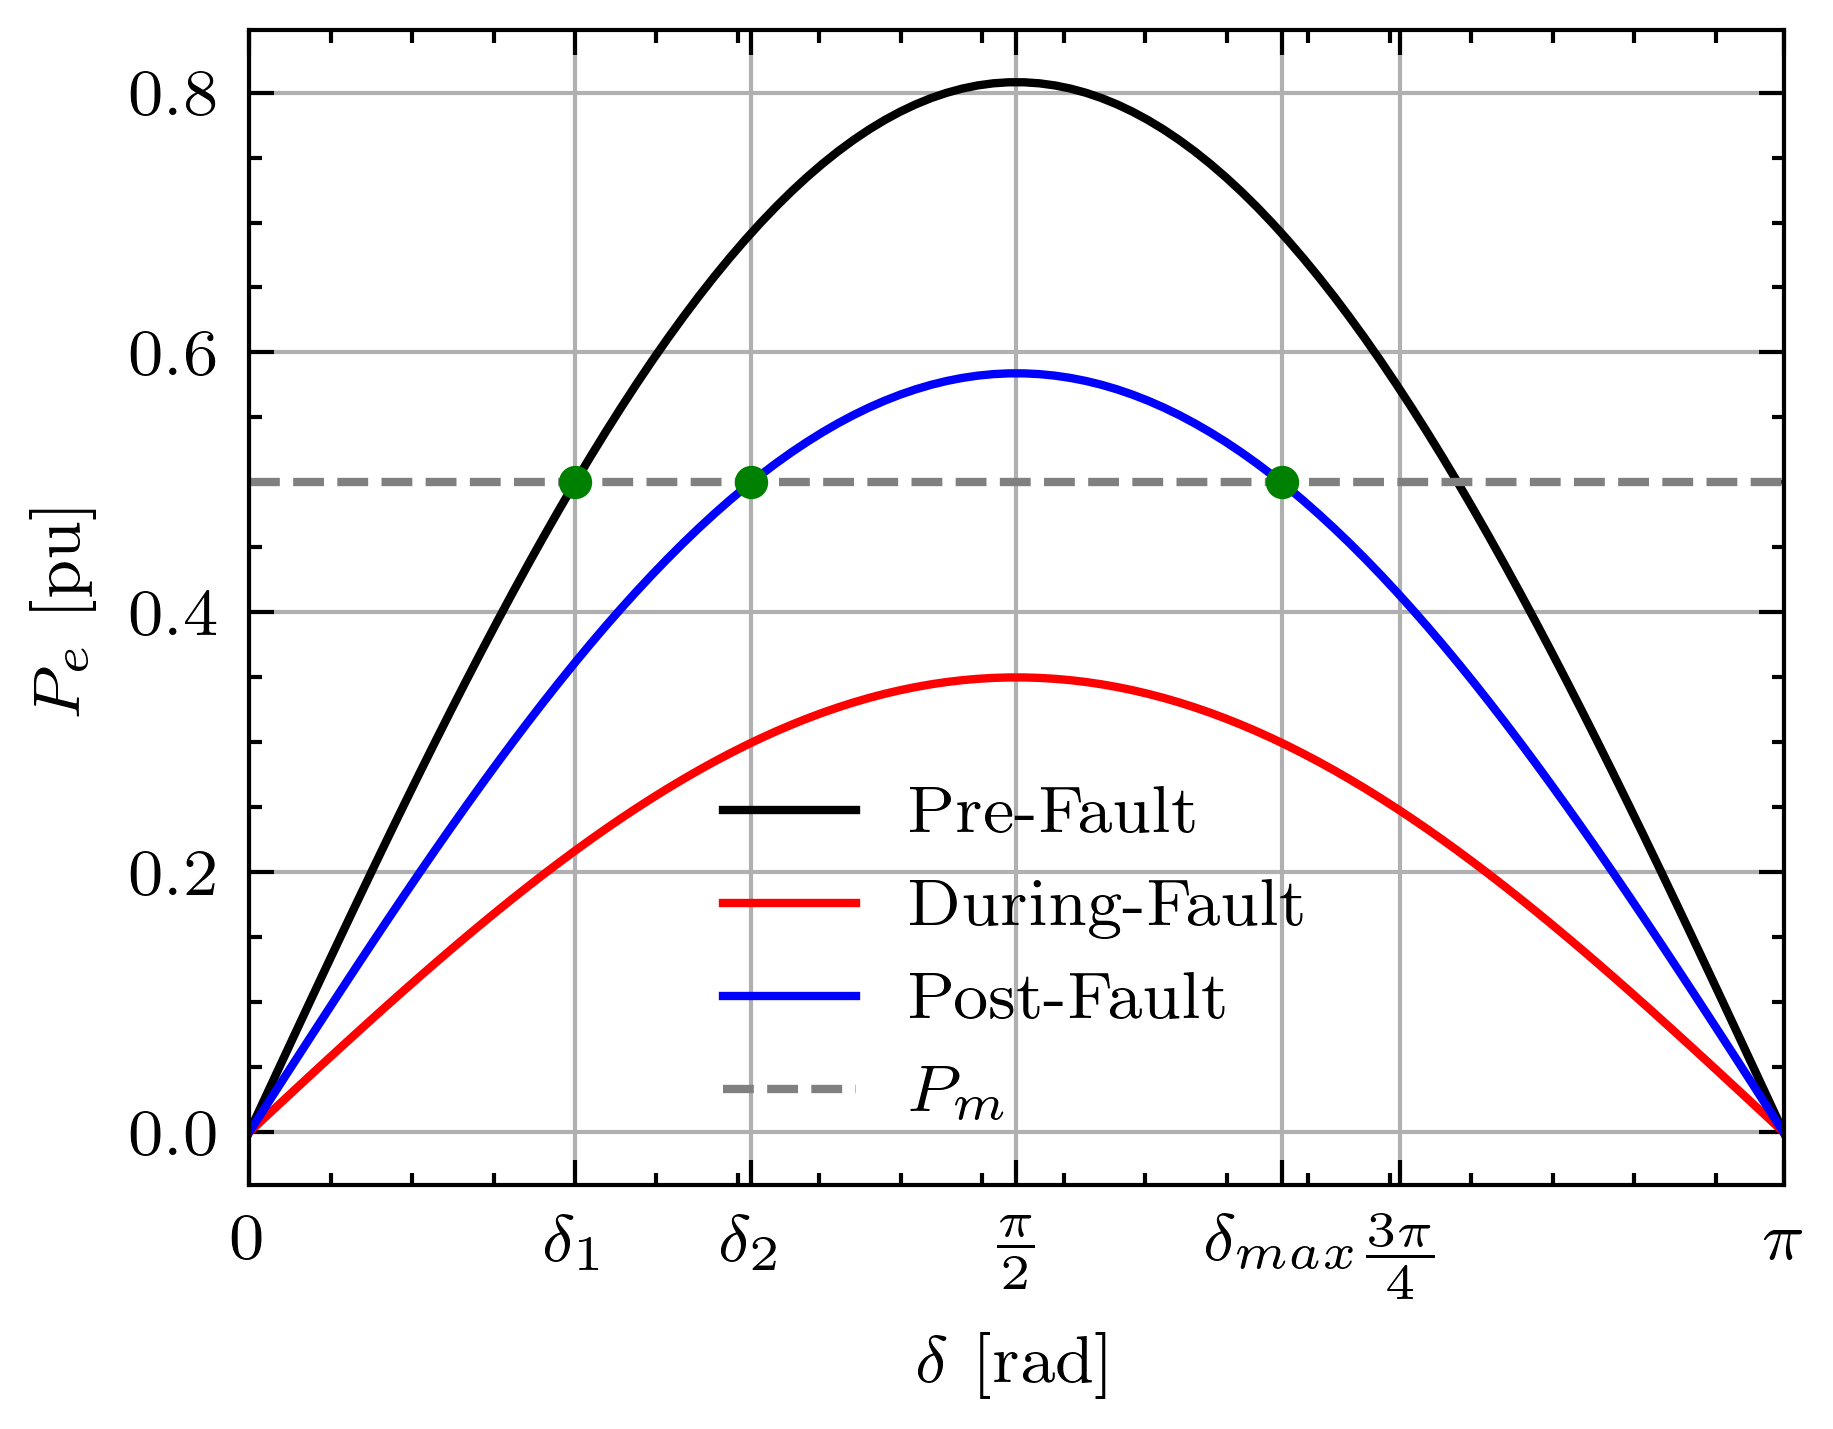
\includegraphics[width=0.95\textwidth]{images/P-delta-example.png}
        \end{center}
    \end{column}
\end{columns}


\end{frame}

\begin{frame}[allowframebreaks]{Critical clearing angle $\delta_{cct}$}
$$\underbrace{\int_{\delta_0}^{\delta_{cct}} \left(P_{m,pu}-P_{e,fault,pu}\right) d\theta}_{\text{Area A}} = \underbrace{\int_{\delta_{cct}}^{\delta_{max}} \left(P_{e,post-fault,pu}-P_{m,pu}\right) d\theta}_{\text{Area B}}$$
\textbf{Area A}
$$
\begin{aligned}
\int_{\delta_{0}}^{\delta_{cct}} \left(P_{m,pu}-P_{e,fault,pu}\right) d\theta &= P_{m,pu} \left(\delta_{cct} - \delta_{0}\right) - \int_{\delta_{0}}^{\delta_{cct}} \hat{P}_{e,df} \sin \theta d\theta \\
&=P_{m,pu} \left(\delta_{cct} - \delta_{0}\right) + \hat{P}_{e,df} \left(\cos \delta_{cct} -\cos \delta_{0}\right) \\
\end{aligned}
$$
\textbf{Area B}
$$
\begin{aligned}
\int_{\delta_{cct}}^{\delta_{max}} \left(P_{e,pf,pu}-P_{m,pu}\right) d\theta &= P_{m,pu} \left(\delta_{cct} - \delta_{max}\right) - \int_{\delta_{cct}}^{\delta_{max}} \hat{P}_{e,pf} \sin \theta d\theta \\
&=P_{m,pu} \left(\delta_{cct} - \delta_{max}\right) + \hat{P}_{e,pf} \left(\cos \delta_{cct} -\cos \delta_{max}\right) \\
\end{aligned}
$$

\textbf{Equal-area criterion}
$$
\begin{aligned}
\text{Area A} &= \text{Area B}\\
P_{m,pu} \left(\delta_{max} - \delta_{0}\right) + \hat{P}_{e,df} \left(\cos \delta_{cct} - \cos \delta_{0}\right) &= \hat{P}_{e,pf} \left(\cos \delta_{cct} - \cos \delta_{max}\right) \\
\end{aligned}
$$
We can find out the critical clearing angle.
$$
\cos \delta_{cct} = \frac{P_{m,pu} \left(\delta_{0} - \delta_{max}\right) + \hat{P}_{e,df} \cos \delta_{0} - \hat{P}_{e,pf} \cos \delta_{max}}{\hat{P}_{e,df} - \hat{P}_{e,pf}}
$$


\begin{columns}
    \begin{column}{0.55\textwidth}
\begin{center}
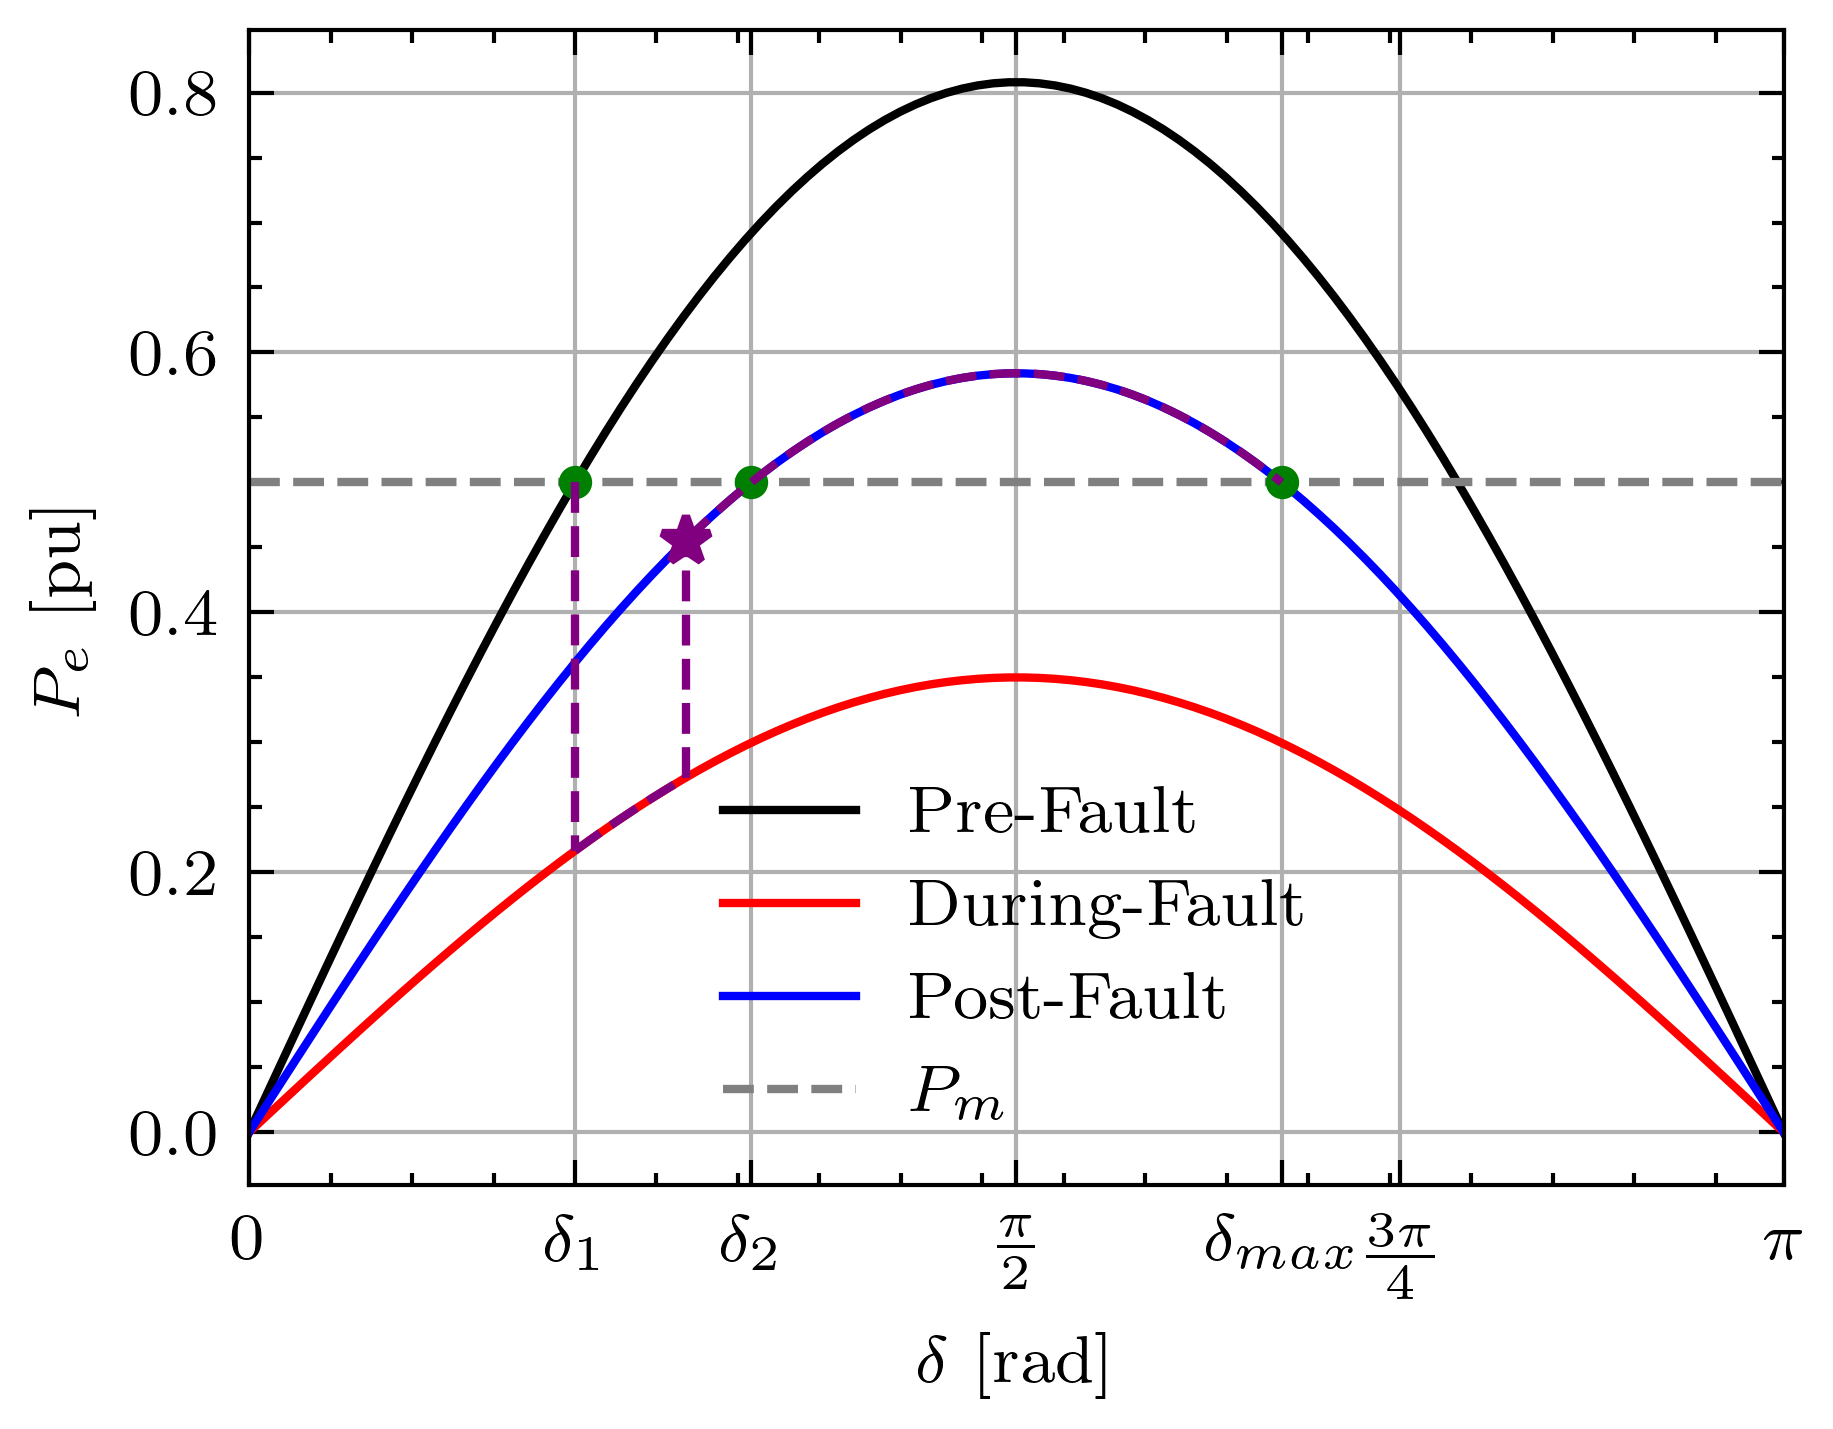
\includegraphics[width=0.8\linewidth]{images/P-delta-example-cct.png}
\end{center}
    \end{column}
    \begin{column}{0.4\textwidth}
The purple star corresponds to $\delta_{cct} = 0.8938$, and the dashed purple line shows the evolution of the angle $\delta$. Even without damping, the system stabilizes at $\delta = \delta_{max}$ since the kinetic energy reaches 0 at that point ($\Delta \omega^2 = 0$)
    \end{column}
\end{columns}

\end{frame}

\begin{frame}[allowframebreaks]{Estimation of the critical clearing time $CCT$}
In order to find the critical clearing time, one would need to solve the swing equation:
$$\left(\frac{2H}{\omega_{syn}}\right) \frac{d^2\delta(t)}{dt^2} = P_{m,pu} - P_{e,pu}(\delta(t))$$
where $P_{e,pu}(\delta(t))$ is a non-linear function depending on $\delta$; $P_{e,pu}(\delta(t)) = K(t) \sin (\delta(t))$, and with $K$ changing non-continuously with time. We would need to solve a non-linear differential equation, which is not an easy task!
Thus, let us assume that the acceleration $\frac{d^2\delta(t)}{dt^2}$ is constant over time. We have:
$$\delta_{cct} = \delta_1 + \Delta \omega_0\ CCT +a \frac{CCT^2}{2}$$
where $a$ is the constant acceleration and $\Delta \omega_0$ the initial speed assumed to be 0.
Let us assume two cases:
\begin{enumerate}
    \item We pick the maximum acceleration for angles in $[\delta_1,\delta_{cct}]$.
    \item We pick the minimum acceleration for angles in $[\delta_1,\delta_{cct}]$.
\end{enumerate}

From the following figure
\begin{center}
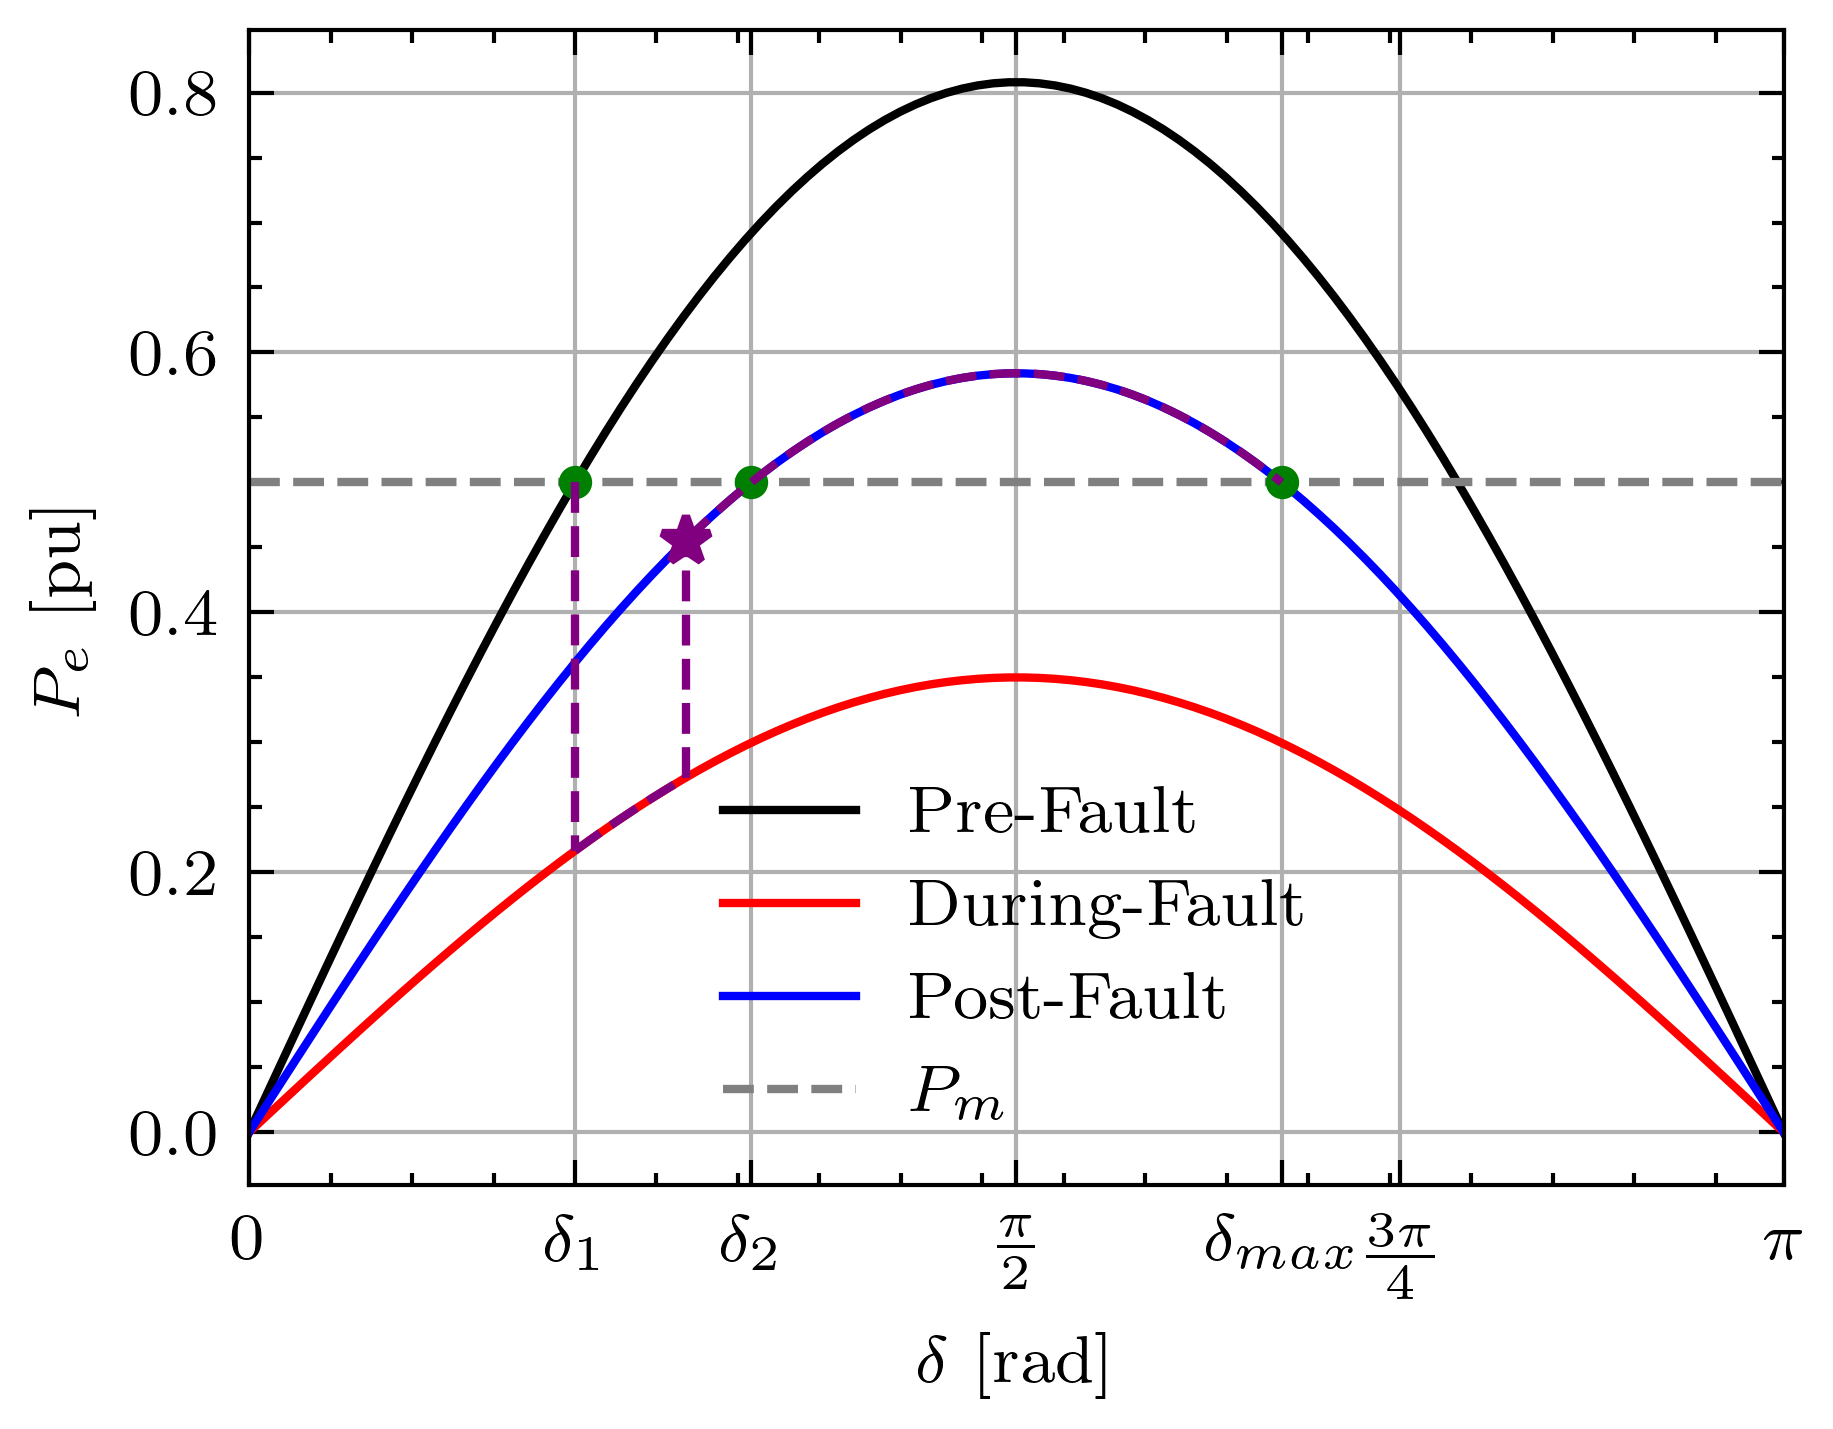
\includegraphics[width=0.6\textwidth]{images/P-delta-example-cct.png}
\end{center}
it is clear that the acceleration is maximum for $\delta = \delta_1$, and minimum for $\delta = \delta_{cct}$ for $\delta \in [\delta_1,\delta_{cct}]$ (larger power mismatch when $\delta = \delta_1$ and smaller for $\delta = \delta_{cct}$).
We have:
$$a_{min} = \frac{\omega_{syn}}{2H}\left(P_{m,pu} - \hat{P}_{e,df}\sin \delta_{cct}\right)$$
$$a_{max} = \frac{\omega_{syn}}{2H}\left(P_{m,pu} - \hat{P}_{e,df}\sin \delta_{1}\right)$$

With $H = 4.5$s, we can derive a lower and an upper bound for the critical clearing time $CCT$.
$$CCT_{max} = \sqrt{\frac{2\left(\delta_{cct}-\delta_{1}\right)}{a_{min}}} = \sqrt{\frac{2\left(0.8938-0.667\right)}{7.93}} = 239 \text{ms}$$
$$CCT_{min} = \sqrt{\frac{2\left(\delta_{cct}-\delta_{1}\right)}{a_{min}}} = \sqrt{\frac{2\left(0.8938-0.667\right)}{9.89}} = 214 \text{ms}$$
If the actual clearing time is denoted $t^*$, we can conclude that:
\begin{enumerate}
    \item If $t^*>CCT_{max}$, the system is unsafe!
    \item If $t^*<CCT_{min}$, the system is safe!
    \item If $CCT_{min}<t^*<CCT_{max}$, we have no guarantee if the system is safe or not.
\end{enumerate}
\end{frame}

\begin{frame} {Extension on dynamics}
\textbf{Swing equations with damping coefficient}
$$\frac{d\Delta \omega(t)}{dt} = \frac{1}{2H}\left(P_m - P_{e,max}(t) \sin (\delta(t)) - D \Delta \omega(t) \right)$$
$$\frac{d\delta(t)}{dt} = \omega_0 \Delta \omega(t)$$
Euler discretization
$$\Delta \omega_{t+1} = (1-\tau \frac{D}{2H})\Delta \omega_{t} + \frac{\tau}{2H}\left(P_m-P_{e,max}^{k \tau}\sin (\delta_{t})\right)$$
$$\delta_{t+1} = \delta_{t} + \tau\omega_0\Delta \omega_t$$
where $\tau$ is the time step and where we explicitly denote that $P_{e,max}^{k \tau}$ is changing over time in a discretize fashion (pre-fault$\rightarrow$during-fault$\rightarrow$post-fault) through the superscript $k \tau$.
\end{frame}

\begin{frame} {Extension on dynamics}
\begin{columns}
    \begin{column}{0.55\textwidth}
        \textbf{Results without damping ($t_{cl} = 0.214 s \leq CCT$)}
        \begin{center}
        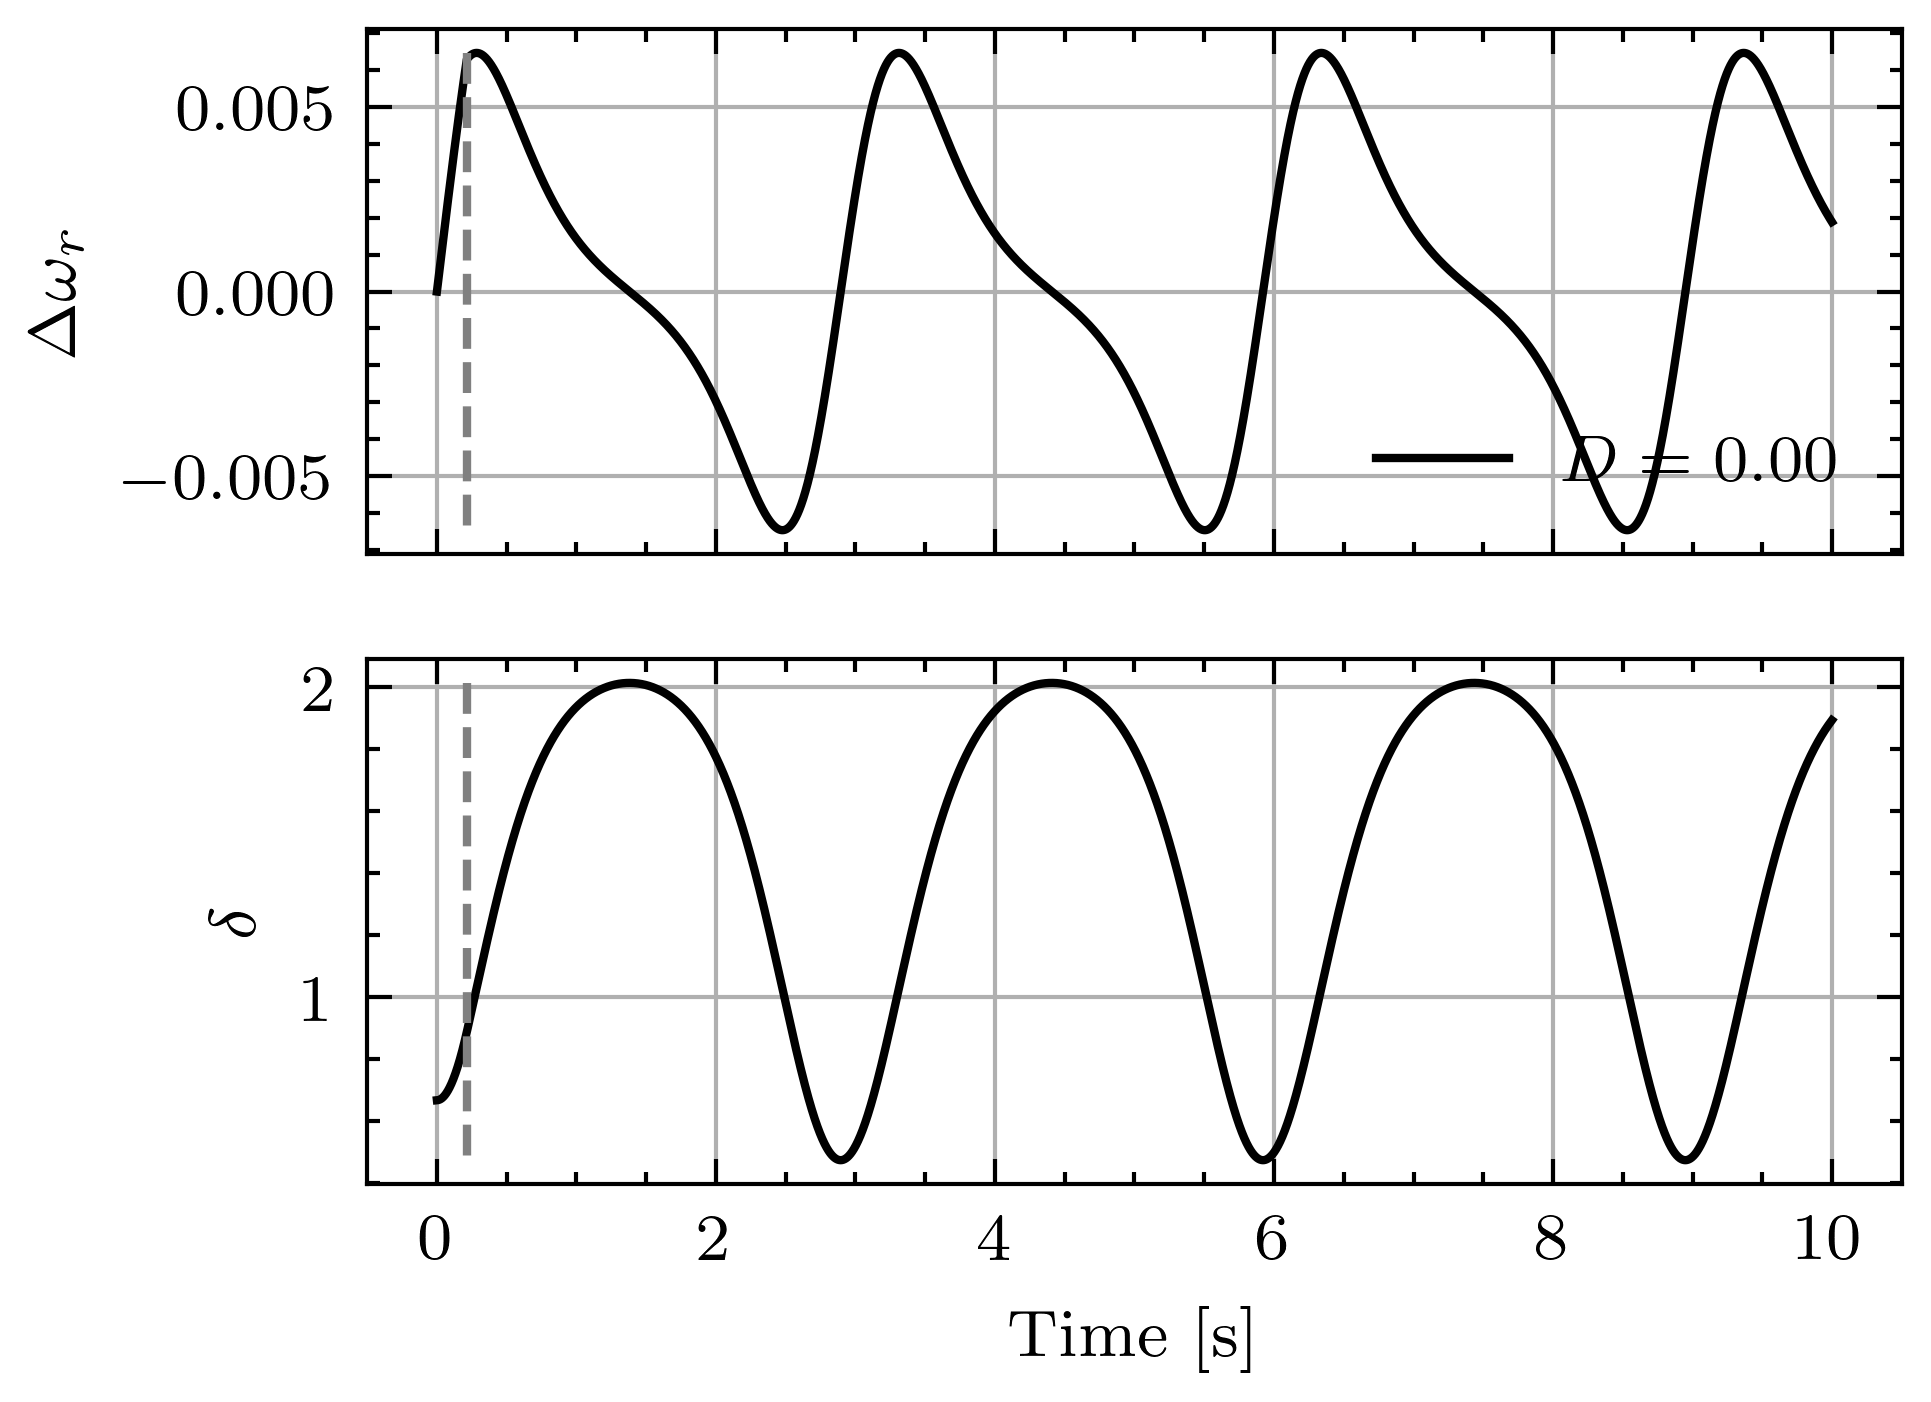
\includegraphics[width=0.9\linewidth]{images/P-dynamics.png}
        \end{center}
    \end{column}
    \begin{column}{0.45\textwidth}
        The fault is cleared after 214 ms (lower bound on the clearing time). As expected from previous calculations, the system is safe.
    \end{column}
\end{columns}
\end{frame}

\begin{frame} {Extension on dynamics}
\begin{columns}
    \begin{column}{0.55\textwidth}
        \textbf{Results with damping ($t_{cl} = 0.214 \leq CCTs$)}
        \begin{center}
        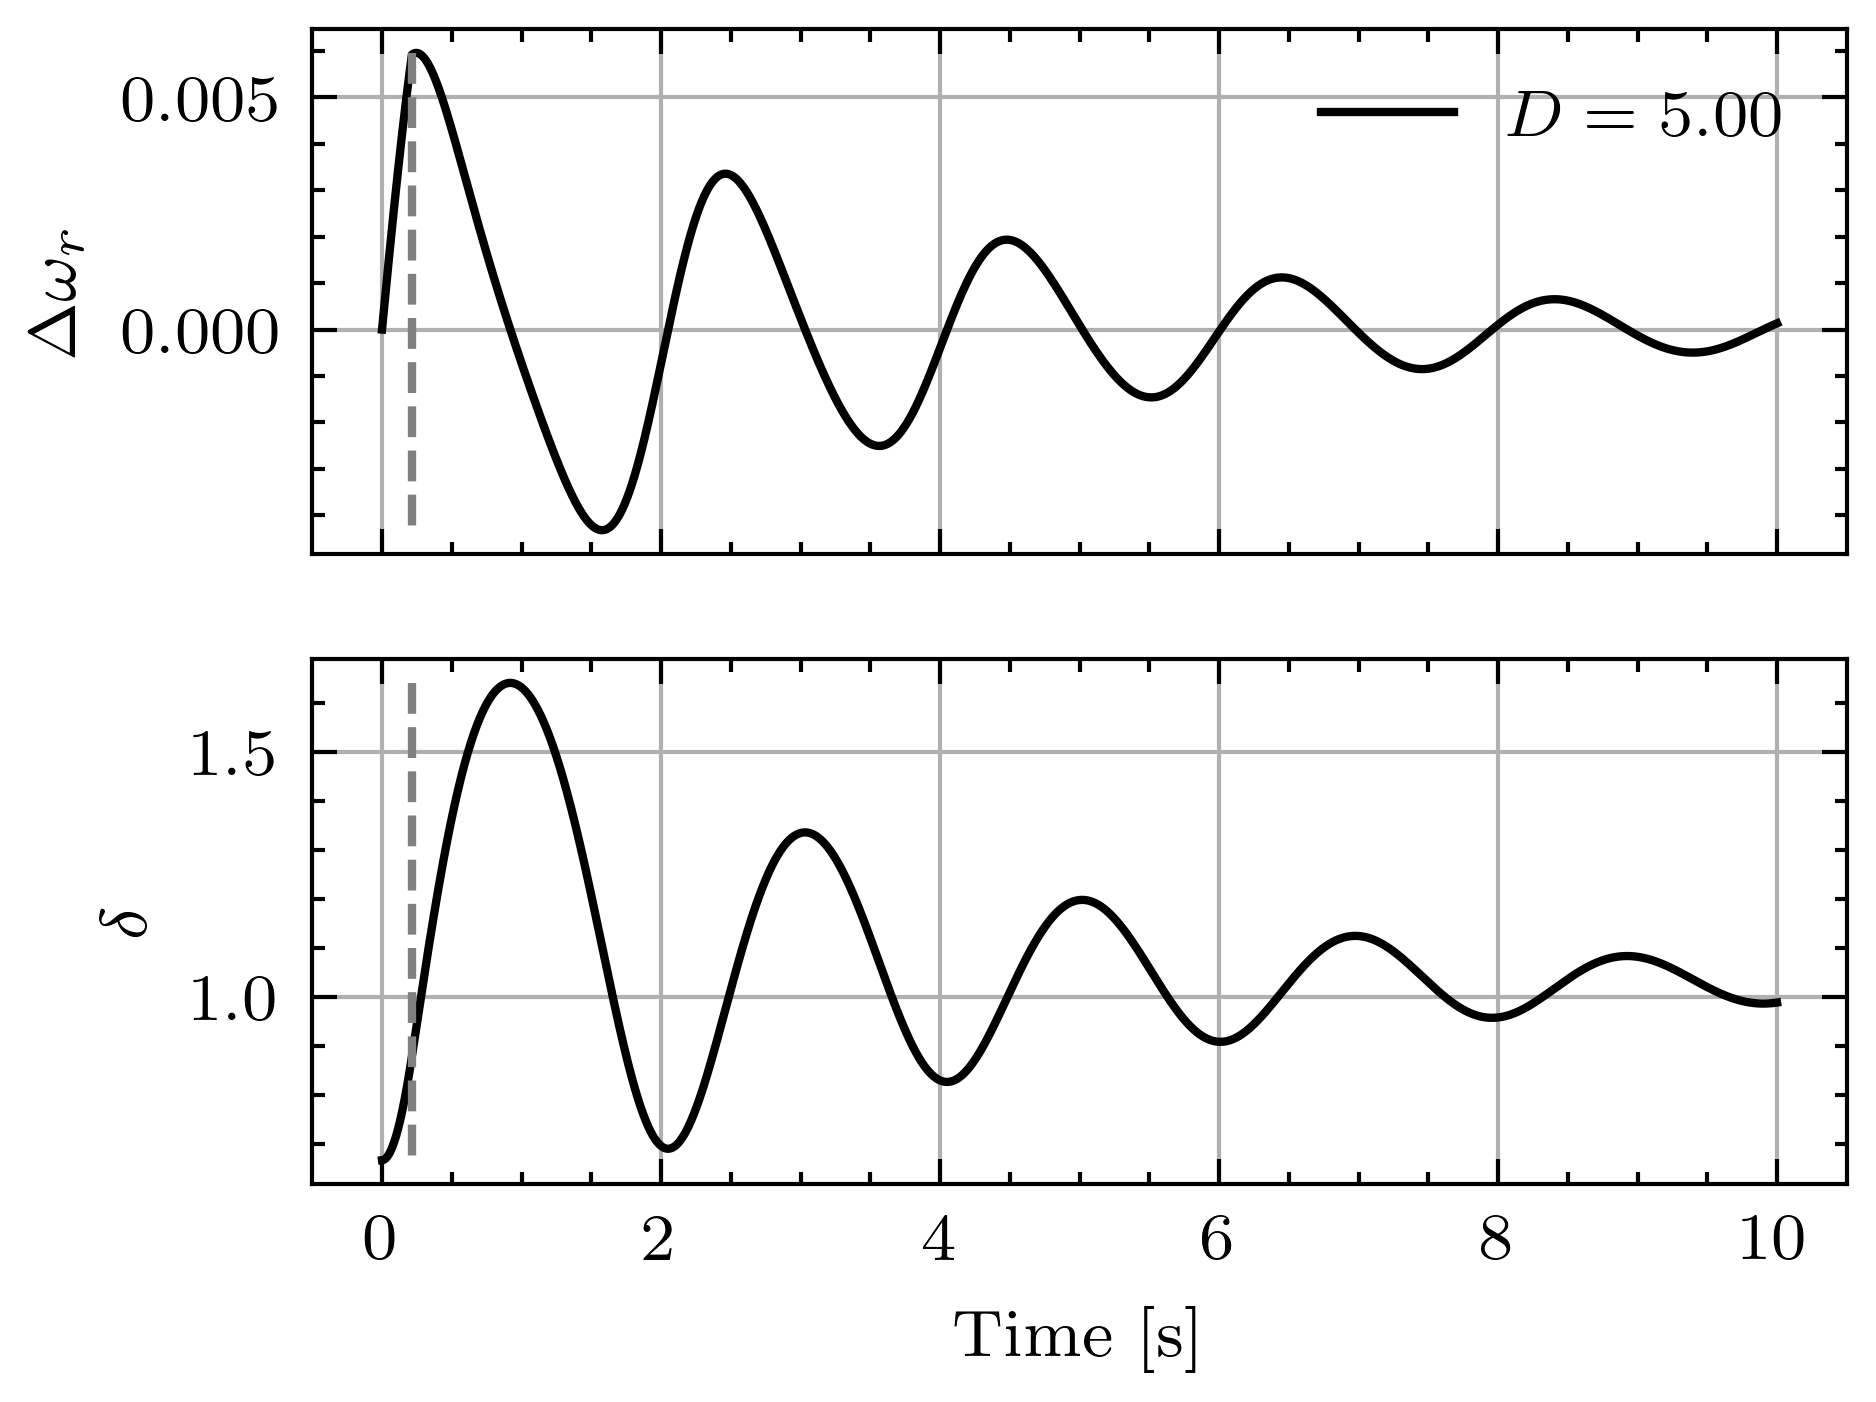
\includegraphics[width=0.9\linewidth]{images/P-dynamics_bis.png}
        \end{center}
    \end{column}
    \begin{column}{0.45\textwidth}
        The fault is cleared after 214 ms (lower bound on the clearing time). As expected from previous calculations, the system is safe. The damping adds energy dissipation, which allows the system to stabilize around $\delta_2 = 1.028$
    \end{column}
\end{columns}
\end{frame}

\begin{frame} {Extension on dynamics}
    \begin{columns}
    \begin{column}{0.55\textwidth}
        \textbf{Results without damping ($t_{cl} = 0.239 s \geq CCT$)}
        \begin{center}
        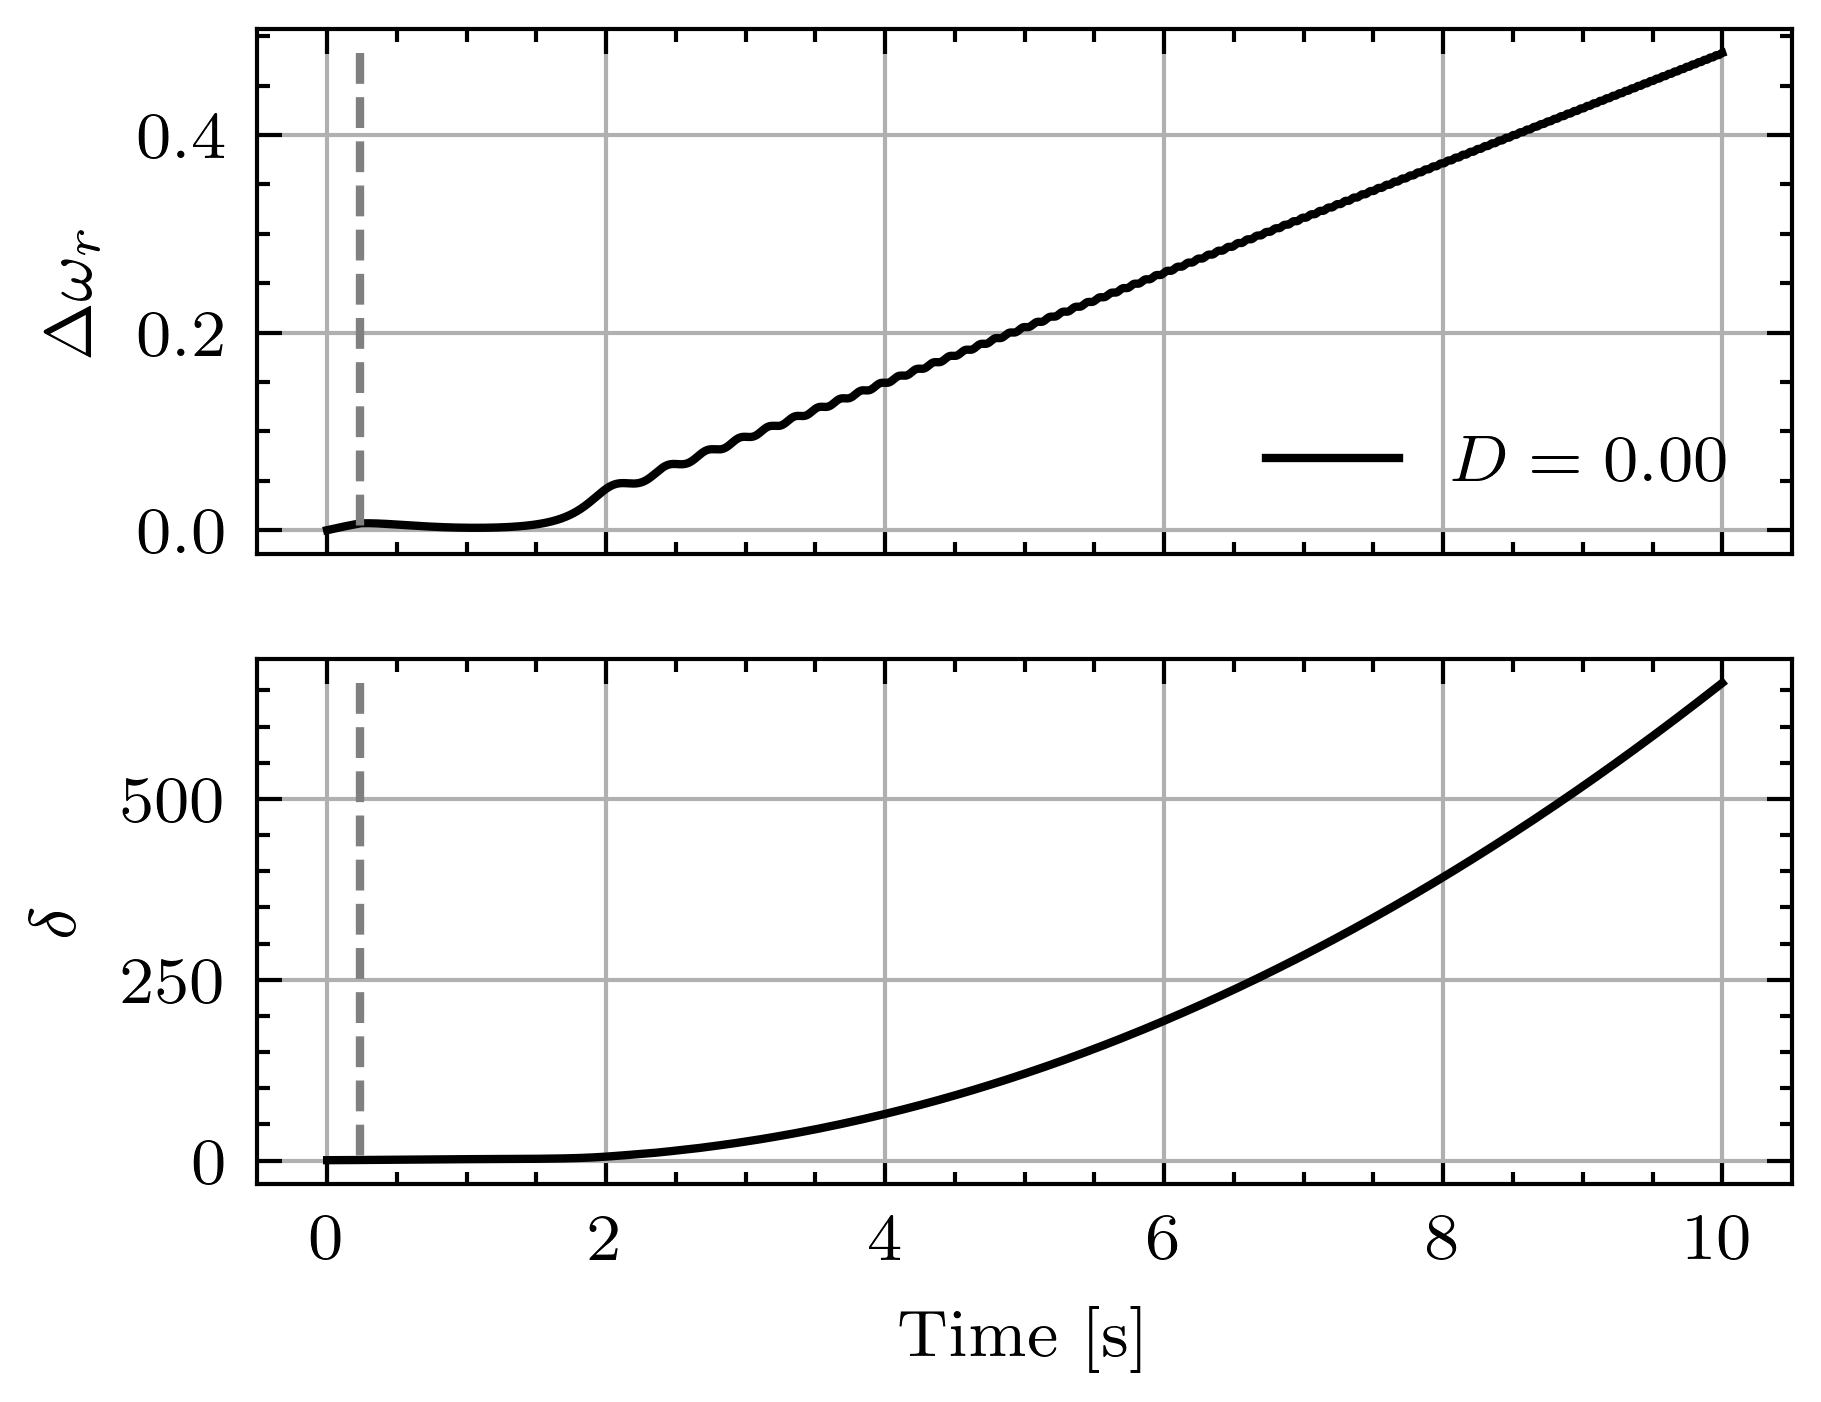
\includegraphics[width=0.9\linewidth]{images/P-dynamics_failed.png}
        \end{center}
    \end{column}
    \begin{column}{0.45\textwidth}
        The fault is cleared after 239 ms (upper bound on the clearing time). The machine loses synchronism.
    \end{column}
\end{columns}

\end{frame}

\begin{frame}{Extension on dynamics}
\begin{columns}
    \begin{column}{0.55\textwidth}
        \textbf{Results with damping ($t_{cl} = 0.239 s \geq CCT$)}
        \begin{center}
        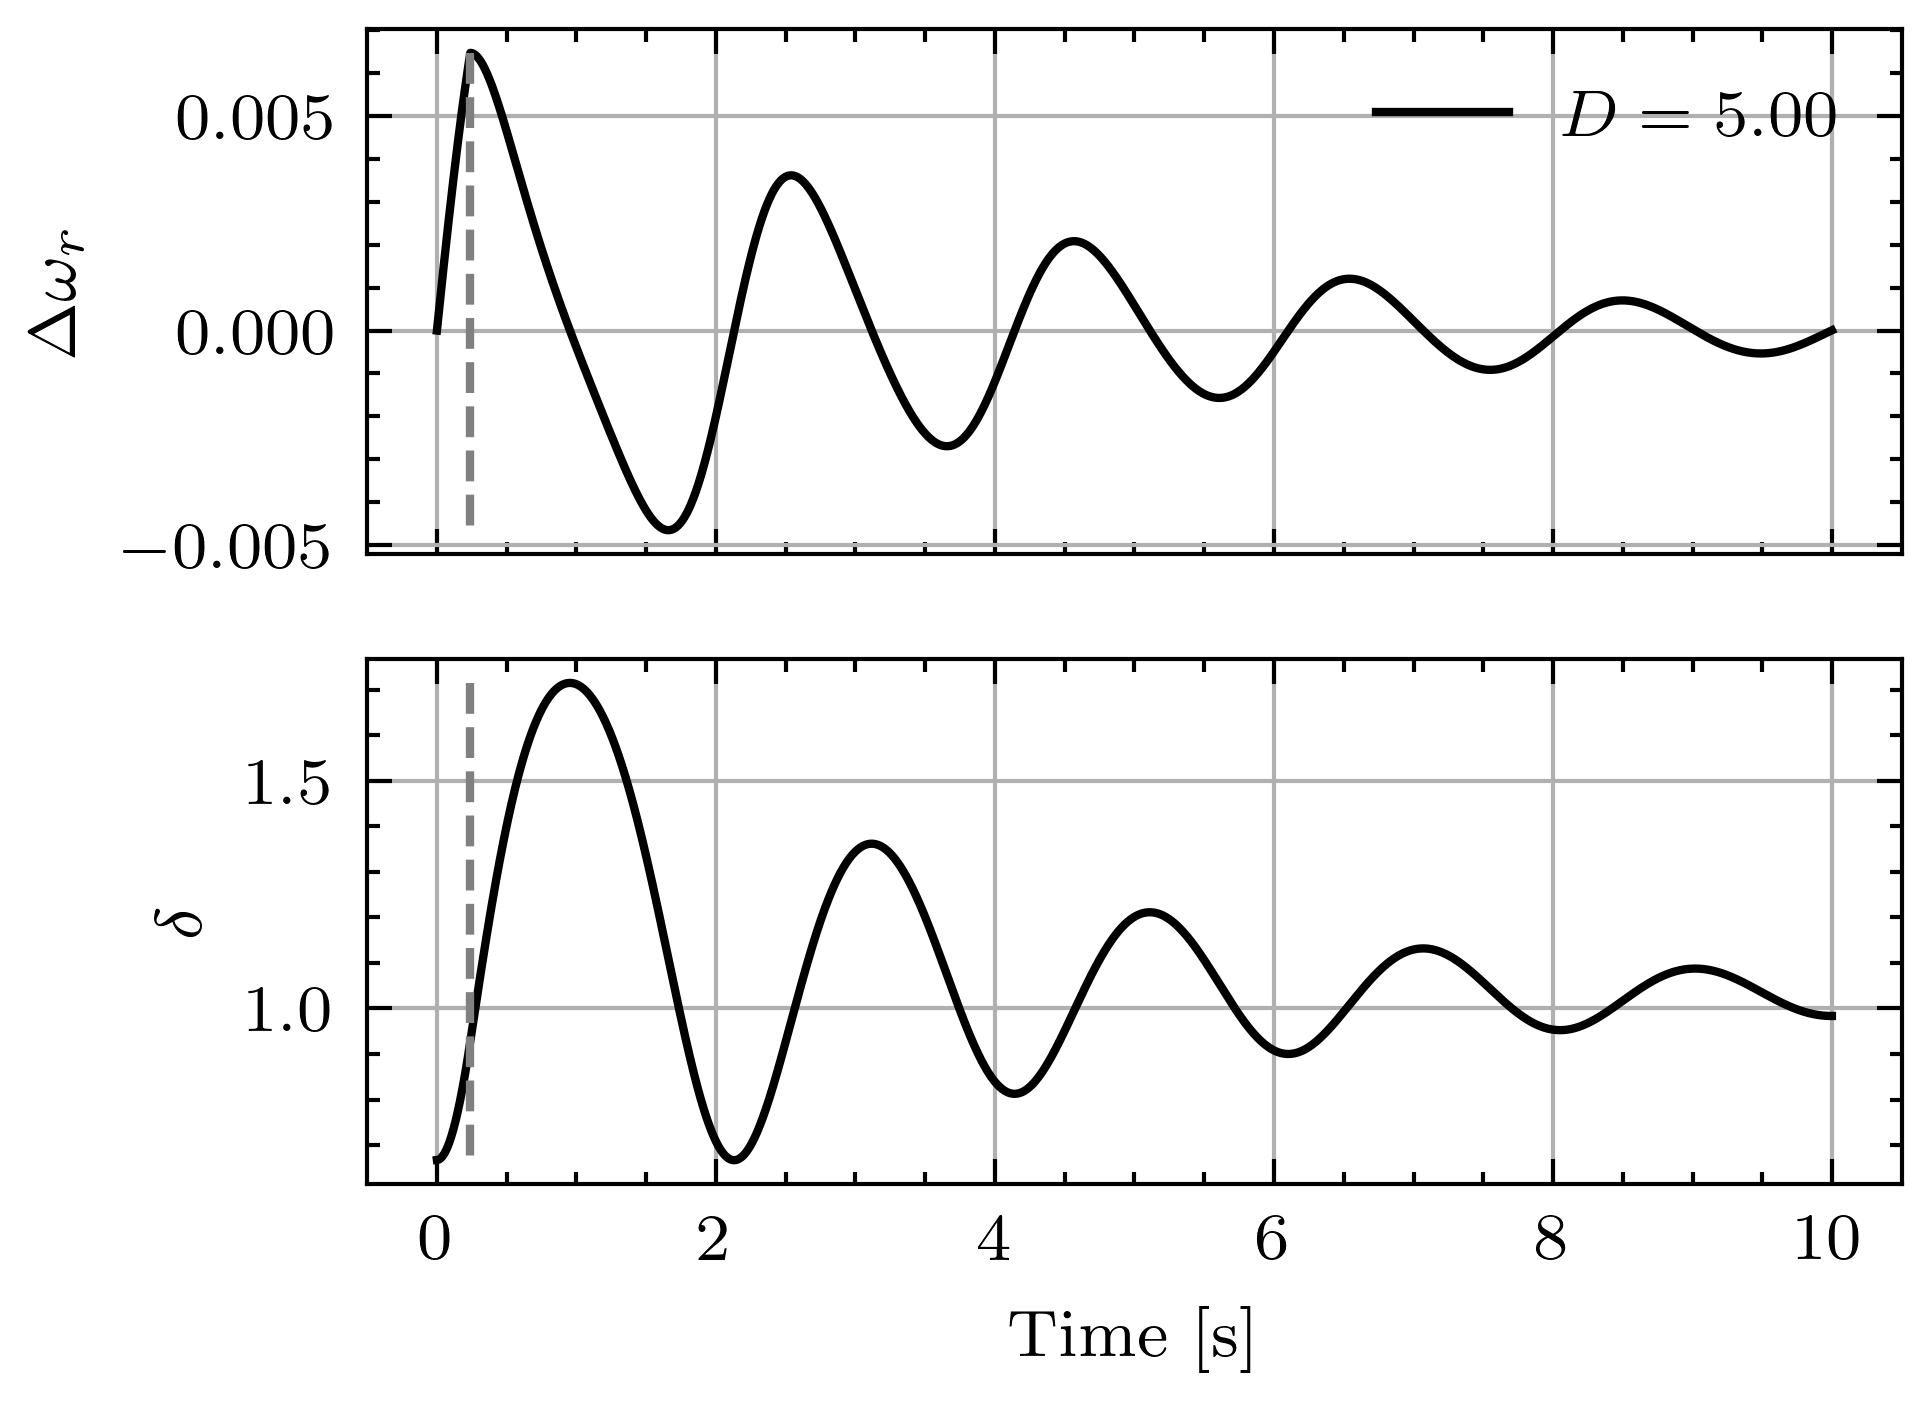
\includegraphics[width=0.9\linewidth]{images/P-dynamics_bis_failed.png}
        \end{center}
    \end{column}
    \begin{column}{0.45\textwidth}
        The fault is cleared after 239 ms (upper bound on the clearing time). The system is stable thanks to the damping effect (energy dissipation).
    \end{column}
\end{columns}
\end{frame}

\section{{Dynamic Security Assessment}}
\begin{frame}{Dynamic Security Assessment goal}

    Main question that Dynamic Security Assessment (DSA) should answer:

\textbf{Imagine a set of major, yet credible contingencies, can the system resist such events without jeopardizing its integrity?}

If yes, then the states are determined secure $\rightarrow$ the system trajectories do not bring the states inside an unsafe set.
\end{frame}

\begin{frame}{Dynamic Security Assessment principle}
\begin{itemize}
    \item Based on fast time domain contingency simulations.
    \item Study main stability issues such that: Voltage, Transient and Small-Signal (not covered throughout this course).
    \item Start from actual and future operating points.
    \item Has to be visual for the operators $\rightarrow$ show the type of instability, where it comes from and even possible solutions.
\end{itemize}
\end{frame}

\begin{frame}{There are mainly types of DSA analysis}
\textbf{1. Off-line analysis}
\begin{itemize}
    \item They are subjected to forecast errors $\rightarrow$ system security cannot be taken for granted.
    \item But they can be performed with no constraints on time (performed day-ahead in order to set up a recommended operating schedule)
\end{itemize}

\textbf{2. On-line analysis}
\begin{itemize}
    \item Not prone to forecast errors since they are based on real-time information.
    \item But need to be fast.
\end{itemize}
\end{frame}

\begin{frame} {Voltage stability assessment}
\begin{columns}
    \begin{column}{0.35\textwidth}
\begin{itemize}
    \item Mainly static analyses.
    \item Goal is to ensure a sufficient load power margin.
    \item List of contingencies: all single-component outages.
\end{itemize}
    \end{column}
    \begin{column}{0.65\textwidth}
        \begin{center}
        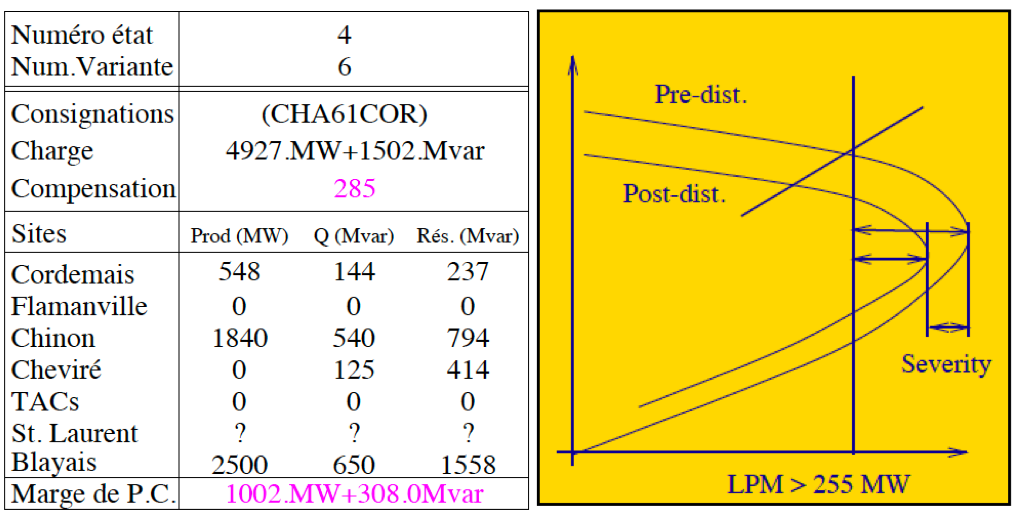
\includegraphics[width=0.9\linewidth]{images/pfonc-sev.png}
        \end{center}
    \end{column}
\end{columns}
\end{frame}

\begin{frame}{Transient stability assessment}
    \begin{columns}
    \begin{column}{0.6\textwidth}
        We want to avoid that:
        \begin{center}
        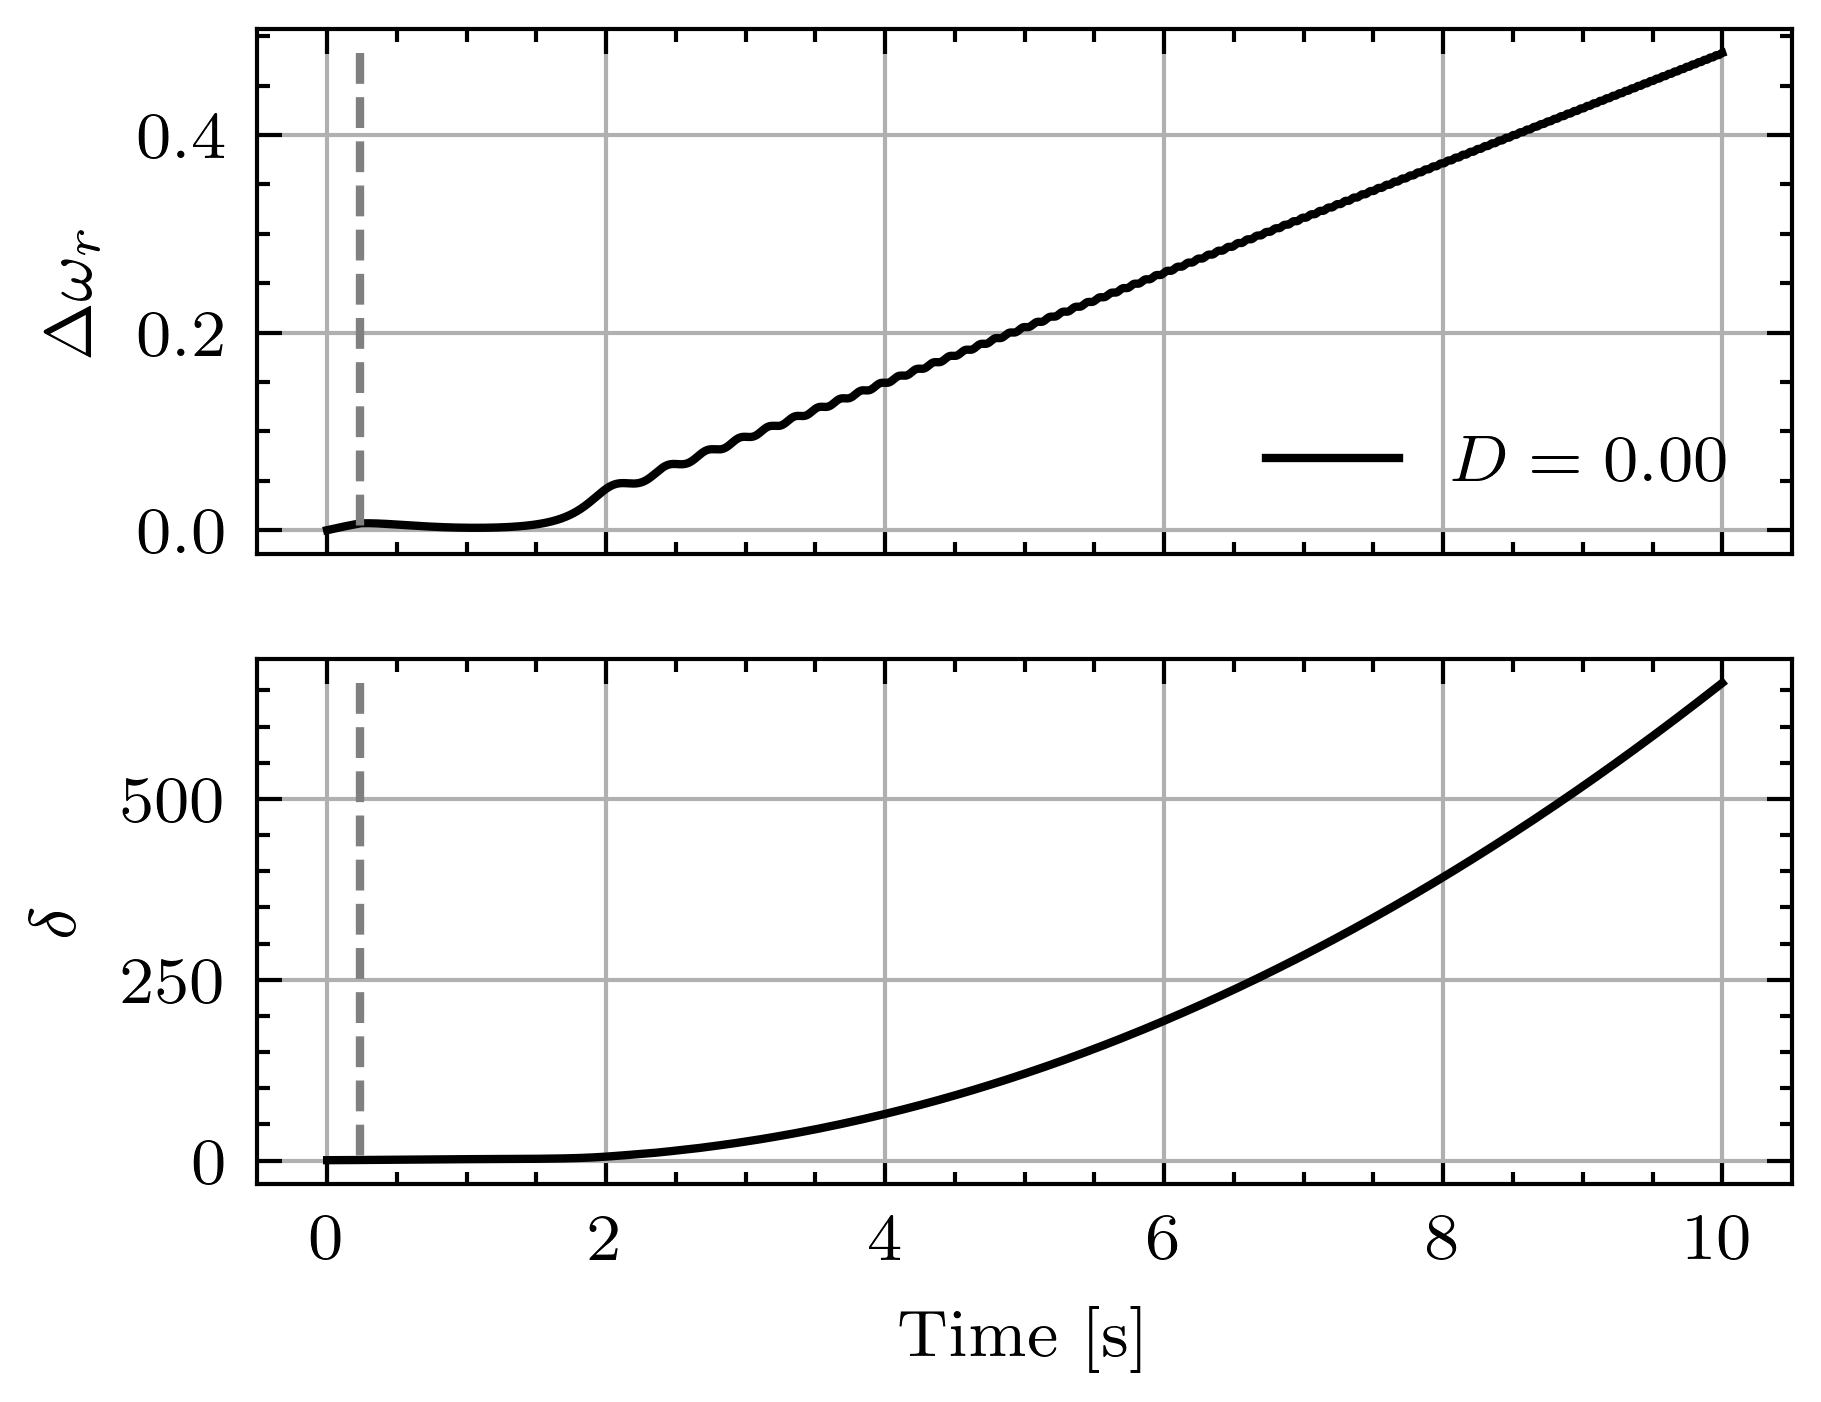
\includegraphics[width=0.9\linewidth]{images/P-dynamics_failed.png}
        \end{center}
    \end{column}
    \begin{column}{0.4\textwidth}
    \begin{itemize}
        \item Simulations with different three-phase short-circuits at various locations.
        \item And with different clearing schemes!
        \item Very time consuming computations.
    \end{itemize}
    \end{column}
\end{columns}
\end{frame}

\section{Trends}
\begin{frame} {Nowadays}
\begin{itemize}
    \item Integration of large off-shore wind parks, and PV systems without reinforcing the network.
    \item Large power plants are decommissioned, and conventional generators are no longer accepted in urban areas.
    \item New units are built far away from load centers.
    \item Hard to build new lines because of public debates and environmental constraints.
\end{itemize}
\emph{This leads to a weaker electrical system, more prone to stability issues.}
There's a need for tools that can quickly perform security assessment to guarantee a secure system.
\end{frame}

\begin{frame}[allowframebreaks]{Example 1: static analysis}
\begin{itemize}
    \item For static analyses, we rely on power flow solvers to estimate the state of the system.
    \item With increasing penetration of RES, probabilistic approaches are envisioned to perform risk assessment.
    \item But traditional power flow solvers based on Newton-Raphson methods are too slow.
    \item Usage of AI tools to derive approximate solutions of the power flow equations.
\end{itemize}
\emph{Donon, B., Clément, R., Donnot, B., Marot, A., Guyon, I., \& Schoenauer, M. (2020). Neural networks for power flow: Graph neural solver. Electric Power Systems Research, 189, 106547.}
\begin{center}
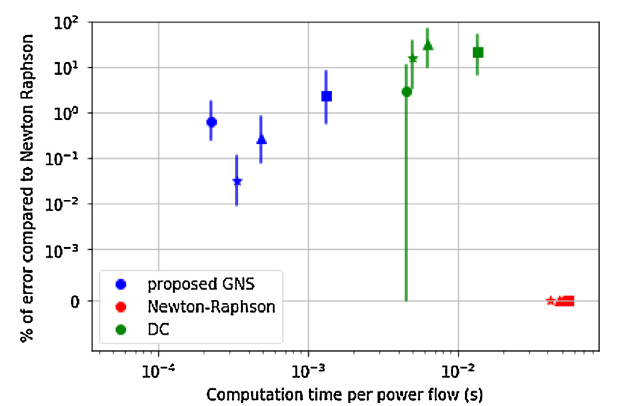
\includegraphics[width=0.7\textwidth]{images/GNS.png}
\end{center}
\end{frame}

\begin{frame}[allowframebreaks]{Example 1: dynamic analysis}
\begin{itemize}
    \item For dynamic analyses, we study the time-evolution of a power system trajectory (e.g. internal angle in transient stability)
    \item It requires solving the differential-algebraic equations for multiple scenarios (different short-circuit locations, different clearing schemes).
    \item Usage of reachability analysis techniques: gives the reach set, i.e., the set that contains all possible system trajectories.
\end{itemize}
\emph{Chen, Y. C., \& Dominguez-Garcia, A. D. (2012). A method to study the effect of renewable resource variability on power system dynamics. IEEE Transactions on Power Systems, 27(4), 1978-1989.}
\begin{center}
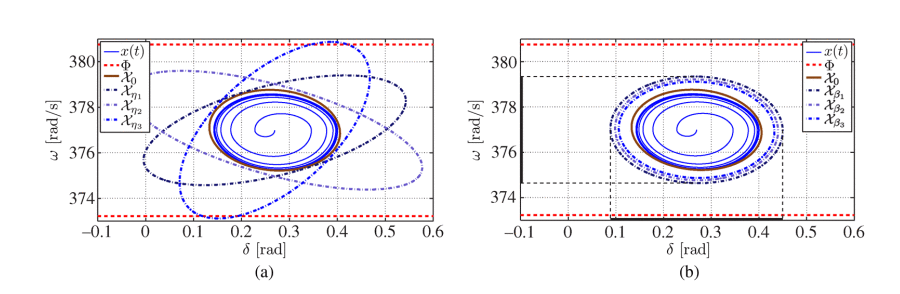
\includegraphics[width=0.95\textwidth]{images/ReachAn.png}
\end{center}
\end{frame}


\end{document}